\section{Selections}
\label{sec:ND280:sel}
The goal of the selection is to map interaction modes (e.g. CCQE, CC1$\pi^+$, CC DIS) to observable ND280 selections, so that theory parameters receive their largest constraints from a few exclusive selections. Equivalent FGD1 and FGD2 selections are separated due to differences in systematics and reconstruction: forward-going tracks emanating in FGD1 leaves a track in FGD1, TPC2, FGD2 and TPC3, so has more hits recorded than the FGD2 equivalence, which only passes through FGD2 and TPC3. Furthermore, FGD2 contains plastic scintillator interleaved with passive water layers whereas FGD1 is fully plastic scintillator. Separating FGD1 and FGD2 also allows constraints on water interactions to come strictly from the FGD2 selections.

The events in the analysis are binned in reconstructed muon candidate variables \pmu and \cosmu. The muon variables are chosen primarily due to excellent detector resolution of muons and for consistency with analyses at SK. There is ongoing effort to include pion variables when such are present (e.g. for CC$1\pi^+$ or CCOther selections), and composite variables in the plane transverse to the neutrino, but will not be presented here.

The selections are entirely defined by the observed reconstructed event topology of an event in the detector and there is no attempt at correcting for misidentified particles. There is no attempt to correct for nuclear effects such as final-state-interactions (FSI).

\subsection{\numu in FHC}
\label{sec:numu_sel}
The different topological selections start by isolating CC-inclusive candidates in FGD1 and FGD2. First, an event is required to contain one reconstructed track of negative charge crossing the TPC downstream of either FGD. The event also needs to fulfil data quality and fiducial volume requirements. The muon is assumed to be the highest momentum negative track (HMNT) found in the event, and it is required that the track is identified as a muon.

The detailed selection criteria for the CC-inclusive sample is:
\begin{itemize}
	\item \textbf{Event quality cut}: The full beam spill has a good global ND280 data quality flag, meaning all ND280 sub-detectors and magnet were operational and reading out data. The event must occur within the bunch time window of the neutrino beam. Event pile-up is mitigated by associating each event to a beam bunch within a beam spill.
	
	\item \textbf{Quality and fiducial volume cut}: At least one reconstructed track is present in the FGD1 or FGD2 fiducial volumes. The fiducial volume for FGD1 is $|x|<874.51\text{ mm}$, $|y-55|<874.51\text{ mm}$, $136.875 < z < 446.955\text{ mm}$ and for FGD2 $|x|<874.51\text{ mm}$, $|y-55|<874.51\text{ mm}$, $1481.45< z < 1807.05\text{ mm}$\footnote{The 55mm offset in $y$ reflects the shift in XY modules relative the center of the ND280 coordinate system.}.
	
	The $x$ and $y$ cuts are designed to accept interactions which have their vertex five bars from the edge of the XY module of each FGD. The $z$ cut excludes the first XY module of each FGD and includes the remaining (14 for FGD1, seven for FGD2). To reject short tracks, for which the TPC reconstruction is unreliable, tracks are required to have more than 18 TPC clusters.
	
	\item \textbf{Upstream background veto}: If the second highest momentum track starts at least 150 mm upstream of the selected muon candidate the event is rejected. This cut eliminates events in which the muon candidate might be the second part of a broken track which started further upstream. For events with a reconstructed vertex in FGD2 there is the added criterion of having no reconstructed tracks in FGD1.
	
	\item \textbf{Broken track cut}: The starting position of the muon candidate track needs to be less than 425 mm away from the FGD upstream edge if the event has at least one reconstructed FGD-only track. The cut vetoes events where the reconstruction has cut a muon candidate track into two tracks: one of which is fully contained in the FGD and the other which starts downstream of the fully contained, misplacing the interaction vertex.
	
	\item \textbf{Muon PID cut}: Once a particle is considered a muon candidate, the particle identification is applied based on the observed $dE/dx$ measurement of the track in the TPC. The measured energy deposit $E$ in the TPC is compared with the expected energy deposit under muon, pion, electron and proton hypotheses and pulls and discrimination functions are applied.
	
	The pulls $\delta_i$ for particle type $i$ are defined as
	\begin{equation}
	\label{eq:tpc_track_chi2}
	\delta_i = \frac{C_T^{obs}-C_T^{exp}}{\sigma^{exp}}
	\end{equation}
	where the expected energy loss $C_T^{exp}$ is parameterised as
	\begin{equation}
	C_T^{exp} = \frac{53.87 \text{ ADC}}{\beta^{2.283}} \left( 5.551 - \beta^{2.283} - \log\left[0.001913 + \frac{1}{\left(\beta\gamma\right)^{1.249}}\right]\right)
	\end{equation}
	$C_T^{obs}$ is the observed energy loss and $\sigma^{exp}$ is the deposited energy resolution of the TPC. ADC refers to the analog to digital counts read out from the detector, indicative of the energy deposited by the particle. $\beta=v/c$ and $\gamma = 1/\sqrt{1-\beta^2}$ are the relativistic variables of the track. The likelihoods $\mathcal{L}_i$ are then defined as
	\begin{equation}
	\label{eq:tpc_track_likelihood}
		\mathcal{L}_i = \frac{e^{-\delta^2_i}}{\sum_n e^{-\delta^2_n}}
	\end{equation}
	where the denominator is summed over the particle types $n=\mu,\pi,e,p$. In the PID algorithm, electrons are rejected by requiring a MIP likelihood
	\begin{equation}
		\label{eq:tpc_track_mip}
		\mathcal{L}_{MIP} = \frac{\mathcal{L}_\mu + \mathcal{L}_\pi}{1-\mathcal{L}_p} > 0.8
	\end{equation}
	for tracks with $p<500\text{ MeV/c}$. To remove protons and pions, it is also required that
	\begin{equation}
	\label{eq:tpc_track_mu}
		\mathcal{L}_\mu > 0.05
	\end{equation}
	The constants 0.8, 0.05 and 500 MeV/c are chosen from particle gun studies in the TPC and test-beam data\cite{t2k_tpc,thesis_tpc, thesis_christine}, and the impact on the selection is shown in \autoref{fig:numu_likelihoods}. The TPC pulls after preselection are shown in \autoref{fig:numu_pulls}, and the energy loss in the TPC from which pulls are derived are shown in \autoref{fig:TPC_dedx}.
	
	Importantly, TPC segments need to pass the TPC track quality cut to contribute to the likelihood: bad quality tracks do not. If a track passes through multiple TPCs all TPC tracks are taken into account.
\end{itemize}

\begin{figure}[h]
	\begin{subfigure}[t]{0.49\textwidth}
		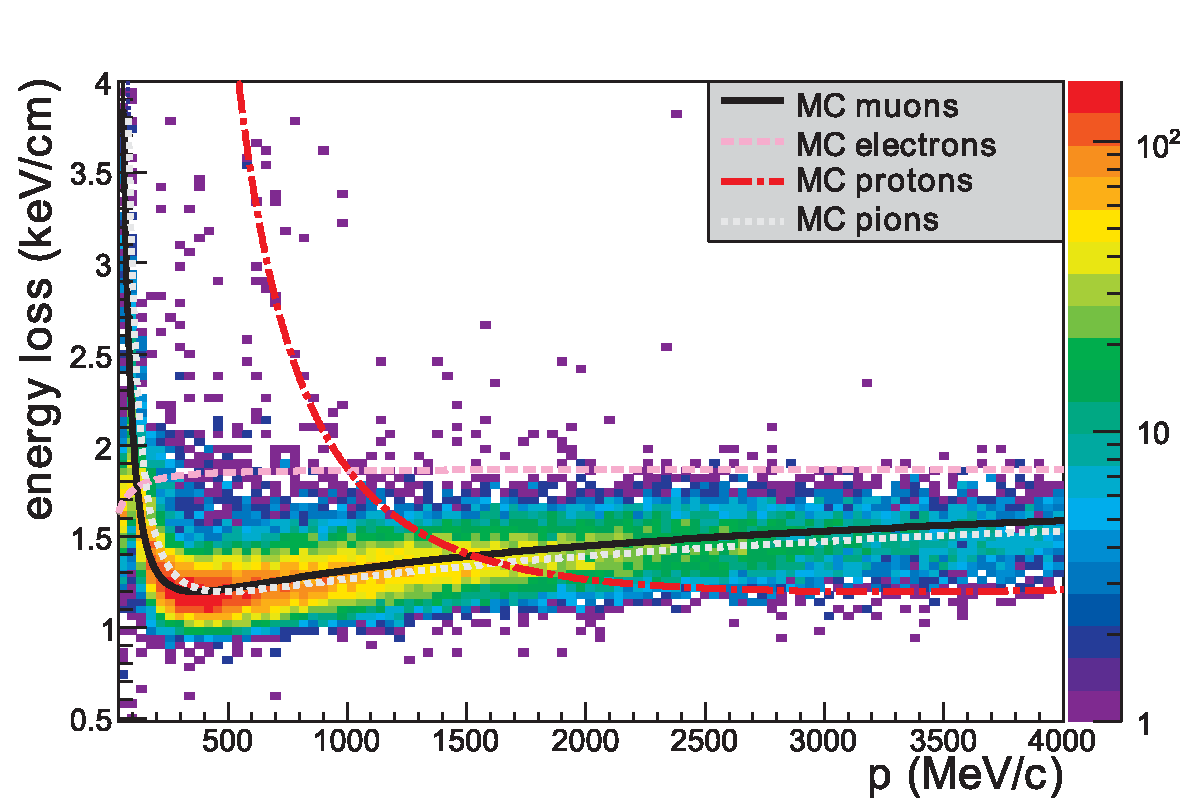
\includegraphics[width=\textwidth]{figures/numu/TPC_PID_neg}
		\caption{Negative particles}
	\end{subfigure}
	\begin{subfigure}[t]{0.49\textwidth}
		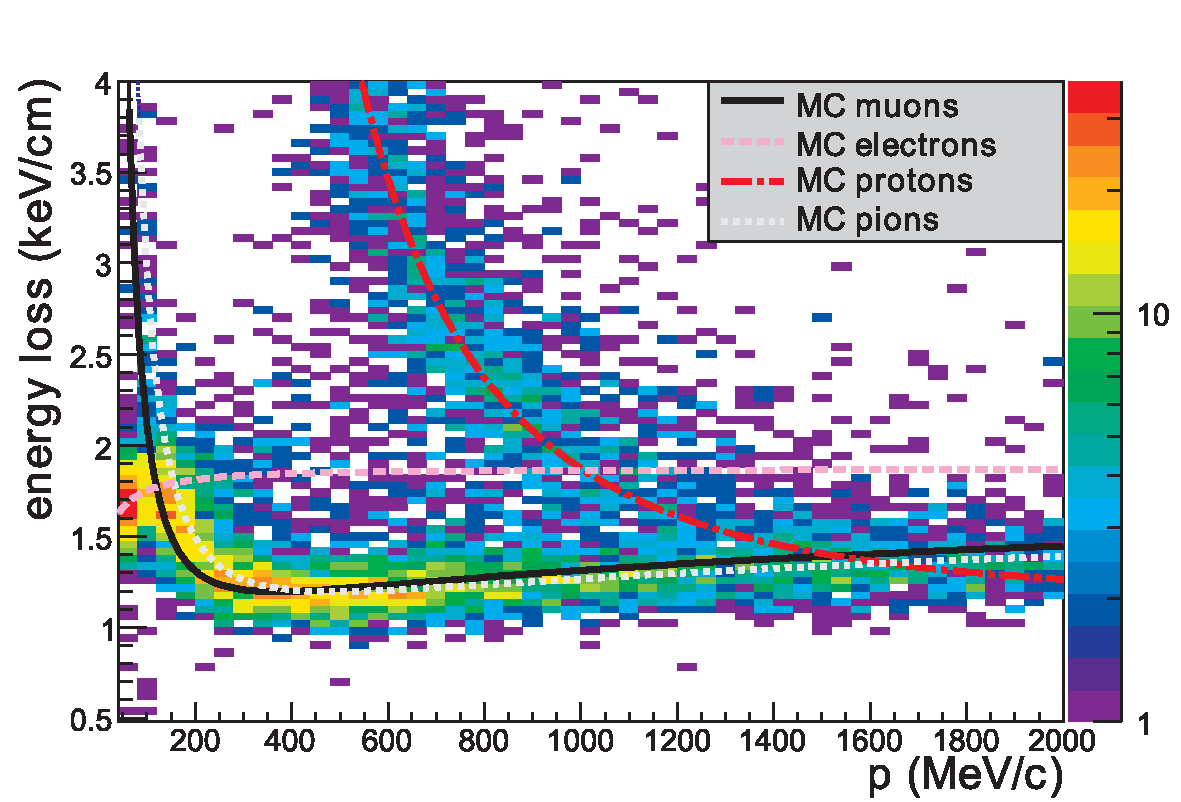
\includegraphics[width=\textwidth]{figures/numu/TPC_PID_pos}
		\caption{Positive particles}
	\end{subfigure}
	\caption{The energy loss for particles travelling through the TPC}
	\label{fig:TPC_dedx}
\end{figure}

\begin{figure}[h]
	\begin{subfigure}[t]{0.49\textwidth}	
		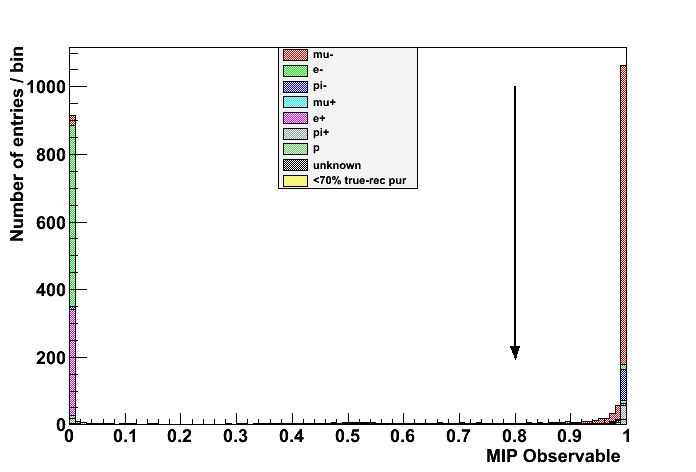
\includegraphics[width=\textwidth]{figures/numu/Cuts/numu/Miplik_run12}
		\caption{$\mathcal{L}_{MIP}$}
	\end{subfigure}
	\begin{subfigure}[t]{0.49\textwidth}	
		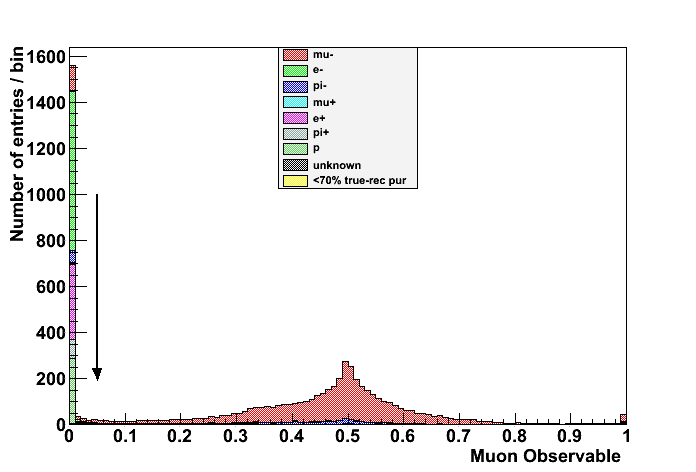
\includegraphics[width=\textwidth]{figures/numu/Cuts/numu/Mulik_run12}
		\caption{$\mathcal{L}_{\mu}$}
	\end{subfigure}
	\caption{Likelihood distributions for preselected MC events, showing cuts placed for \numu in FHC analysis}
	\label{fig:numu_likelihoods}
\end{figure}

\begin{figure}[h]
	\begin{subfigure}[t]{0.32\textwidth}
		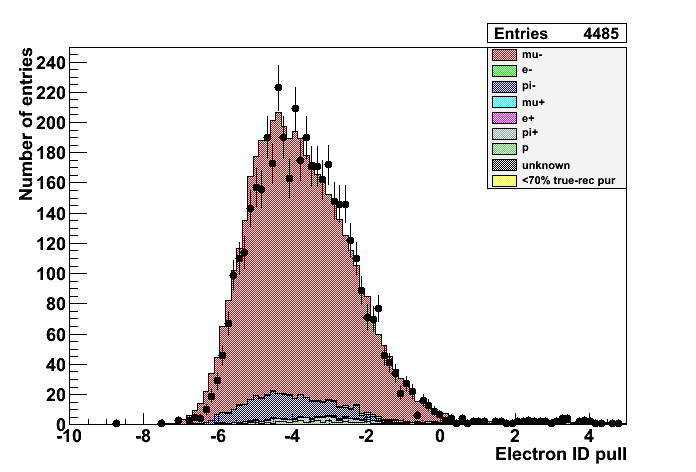
\includegraphics[width=\textwidth]{figures/numu/Cuts/numu/Elepull_run12}
		\caption{$\delta_e$}
	\end{subfigure}
	\begin{subfigure}[t]{0.32\textwidth}	
		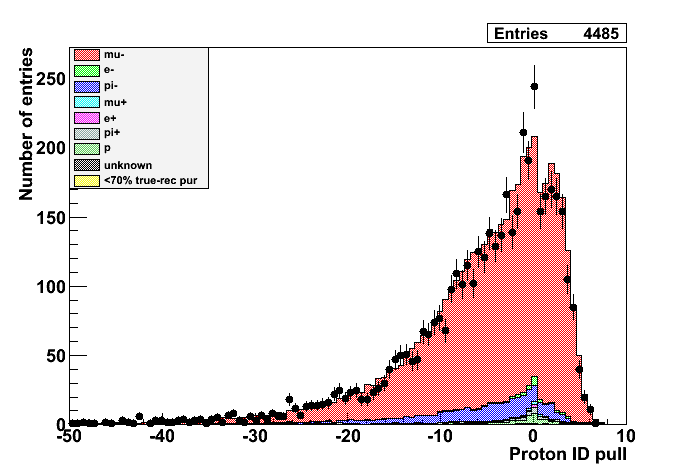
\includegraphics[width=\textwidth]{figures/numu/Cuts/numu/Protpull_run12}
		\caption{$\delta_p$}
	\end{subfigure}
	\begin{subfigure}[t]{0.32\textwidth}
		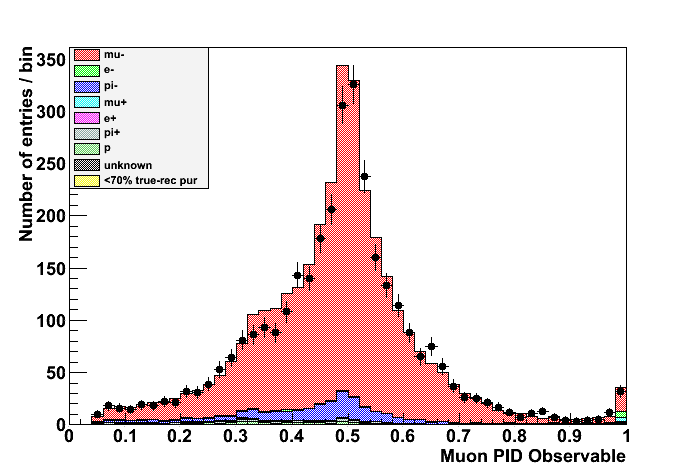
\includegraphics[width=\textwidth]{figures/numu/Cuts/numu/Mulikelihood_run2}
		\caption{$\delta_\mu$}
	\end{subfigure}
	\caption{Pull distributions after selection showing data and MC for \numu analysis}
	\label{fig:numu_pulls}
\end{figure}

The selection criteria proceeds to split the CC-inclusive sample into the three subsamples: CC$0\pi$, CC$1\pi$ and CCOther. This is based entirely on pion identification in the TPCs and FGDs. To identify pion candidate(s) a number of cuts are applied:
\begin{itemize}
	\item \textbf{Muon candidate}: The track can not be identified as the above muon candidate.
	
	\item \textbf{Matching beam spill and bunch}: The pion candidate is required to originate from the same beam bunch and spill to the identified muon candidate.
	
	\item \textbf{Track origin}: The pion candidate is required to start in the same FGD fiducial volume as the muon candidate and enter the downstream TPC for PID purposes. The same FGD and TPC track quality and fiducial volume cut is applied for the pion candidate as for the muon candidate.
	
	\item \textbf{Pion PID}: For positive tracks in the TPC, pion, positron and proton hypotheses are tested. For negative tracks, pion and electron hypotheses are tested. 
	
	As for the muon candidate, \autoref{eq:tpc_track_chi2} and \autoref{eq:tpc_track_likelihood} define the particle likelihoods. For the pion PID, the MIP likelihood in \autoref{eq:tpc_track_mip} is required and in addition a cut on the pion likelihood is invoked,
	\begin{equation}
	\label{tpc_track_pi}
		\mathcal{L}_\pi > 0.3
	\end{equation}
	
	When there is no particle track in the TPC, the FGD PID is used to count the number of charged pions. However, it can not be used for neutral pions because there is currently no electron or positron reconstruction available in the FGD. The FGD pion PID proceeds either by:
	\begin{itemize}
		\item \textbf{Michel electron tag}: A search for a Michel electron tag is made for low-momentum tracks that fail to leave enough hits for track reconstruction. It looks for a time-delayed FGD hit cluster out of time with a beam bunch window. A Michel candidate is found if the number of hits in the delayed time bin is greater than six for FGD1 and five for FGD2\footnote{Roughly corresponding to 200 photoelectrons, which can't be used as a criteria in FGD2 due to the water layers}. Since there is no measurement of the track, the pion has no associated momentum or angle.
		
		\item \textbf{FGD reconstruction}: Higher momentum pions may leave fully contained tracks in the FGD. If such a track belongs to the same bunch as the muon candidate and there is only one pion track reconstructed in the FGD, it is considered a pion candidate. The pion candidate is required to be upwards or downwards-going by invoking $|\cos\theta_{\pi,\nu}| > 0.3$, which limits the possibility of travelling along the FGD bars. Finally we require a pion pull of $-2 < P_\pi < 2.5$ in the FGD from its track length, shown in \autoref{fig:FGD_pion_pulls}.
	\end{itemize}
\end{itemize}
\begin{figure}[h]
	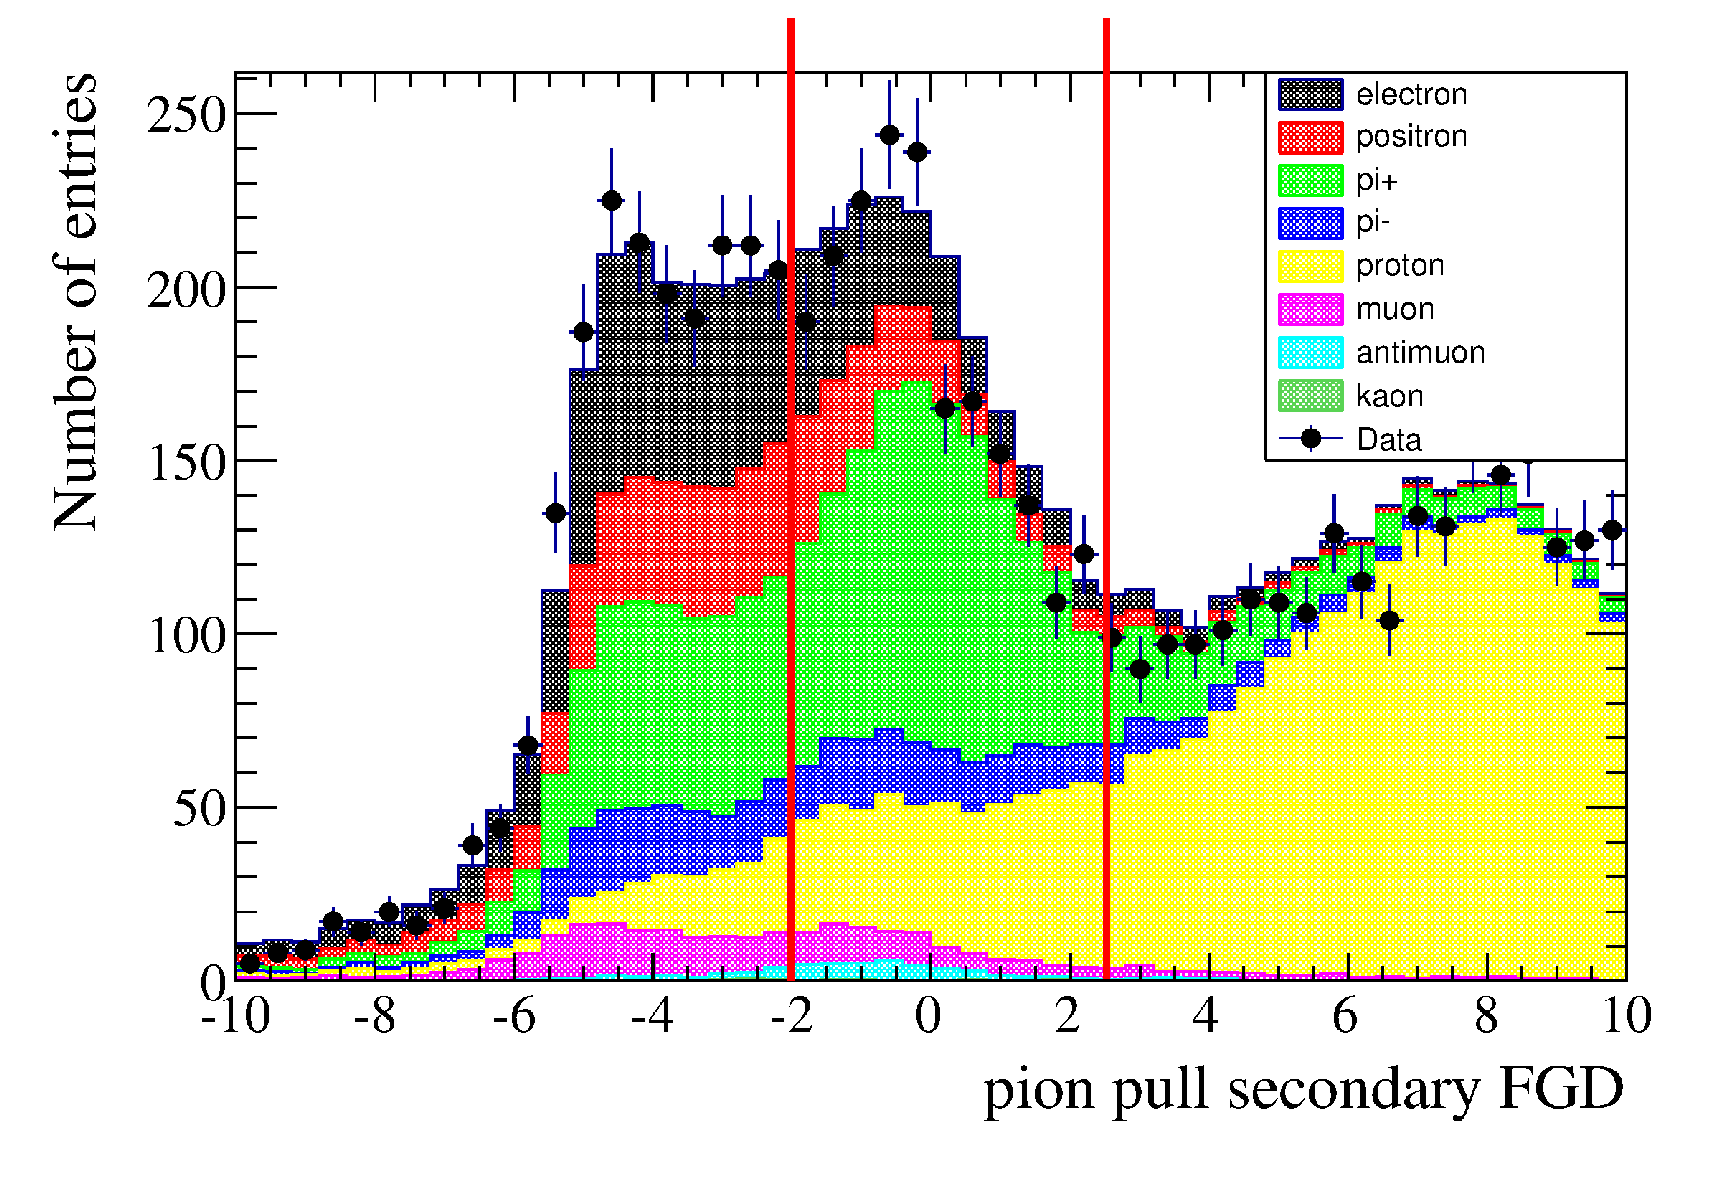
\includegraphics[width=0.5\textwidth]{figures/numu/Cuts/pull_secondarytrack_FGD_all.eps}
	\caption{FGD1 pion pulls for a fully contained track}
	\label{fig:FGD_pion_pulls}
\end{figure}

Finally, the remaining particles can be identified using the TPC PID: 
\begin{itemize}
	\item For a positive particle, it is tagged according to highest probability. If the most likely particle is a positron but the $p_{reco} > 900\text{ MeV}$ it's tagged as a proton, otherwise it is a positron.
	
	\item For a negative particle, if the probability of a pion is $P_\pi>0.8$ it is tagged as a negative pion, and if not it is assumed an electron.
\end{itemize}

Using information from the TPC PID, FGD Michel electron and FGD PID algorithms, the \numu CC-inclusive sample is categorised into the CC$0\pi$, CC$1\pi$ and CCOther samples:
\begin{itemize}
	\item \textbf{CC0$\pi$}: Contains events with one negative muon candidate, no identified charged or neutral pions in the TPC or FGD, and no electrons or positrons in the TPC. The selection predominantly contains CCQE and 2p2h events and is the largest sample at ND280. An example event display is shown in \autoref{fig:cc0pi_evtdisplay}.
	\begin{figure}[h]
		\begin{subfigure}[t]{0.49\textwidth}
			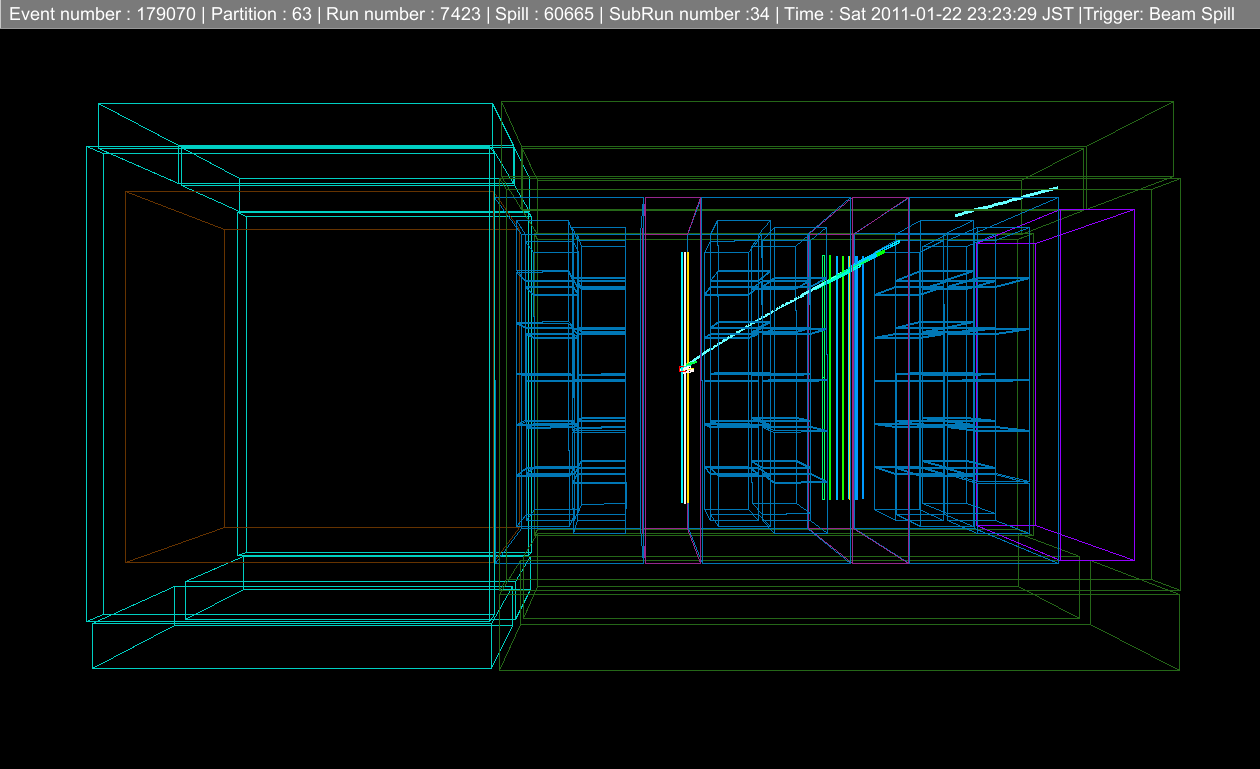
\includegraphics[width=\textwidth, trim={25mm 28mm 30mm 30mm}, clip]{figures/numu/evtdisplay/CC0pi_7423_34_179070_perX0Z_all}
			\caption{Side-view}
		\end{subfigure}
		\begin{subfigure}[t]{0.49\textwidth}
			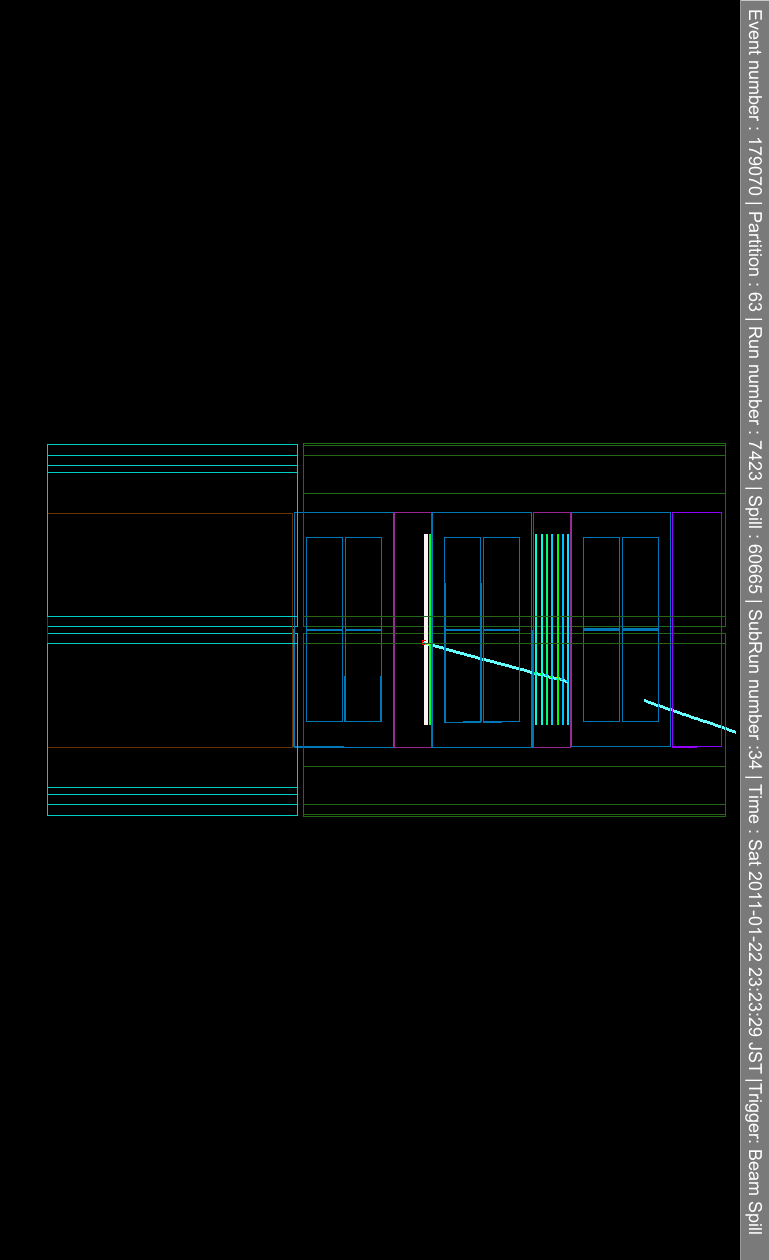
\includegraphics[width=\textwidth, trim={10mm 150mm 10mm 150mm}, clip]{figures/numu/evtdisplay/CC0pi_7423_34_179070_ortX0Z_all}
			\caption{Top-view}
		\end{subfigure}
		\caption{True FGD1 CC0$\pi$ event display in ND280}
		\label{fig:cc0pi_evtdisplay}
	\end{figure}

	\item \textbf{CC$1\pi$}: Contains events with one negative muon candidate and one positive pion candidate. The sum of the number of positive pions found in the TPC and the number of Michel electrons is one and if there are no Michel electrons the sum of positive pions in the TPC and fully contained in the FGD is one. If there is a negative pion, electron or positron reconstructed in the TPC it is rejected. The selection contains mostly CC1$\pi^{+}$ and multi-$\pi^+$ events from resonant and DIS interactions. An example event display is shown in \autoref{fig:cc1pi_evtdisplay}.
	\begin{figure}[h]
		\begin{subfigure}[t]{0.49\textwidth}
			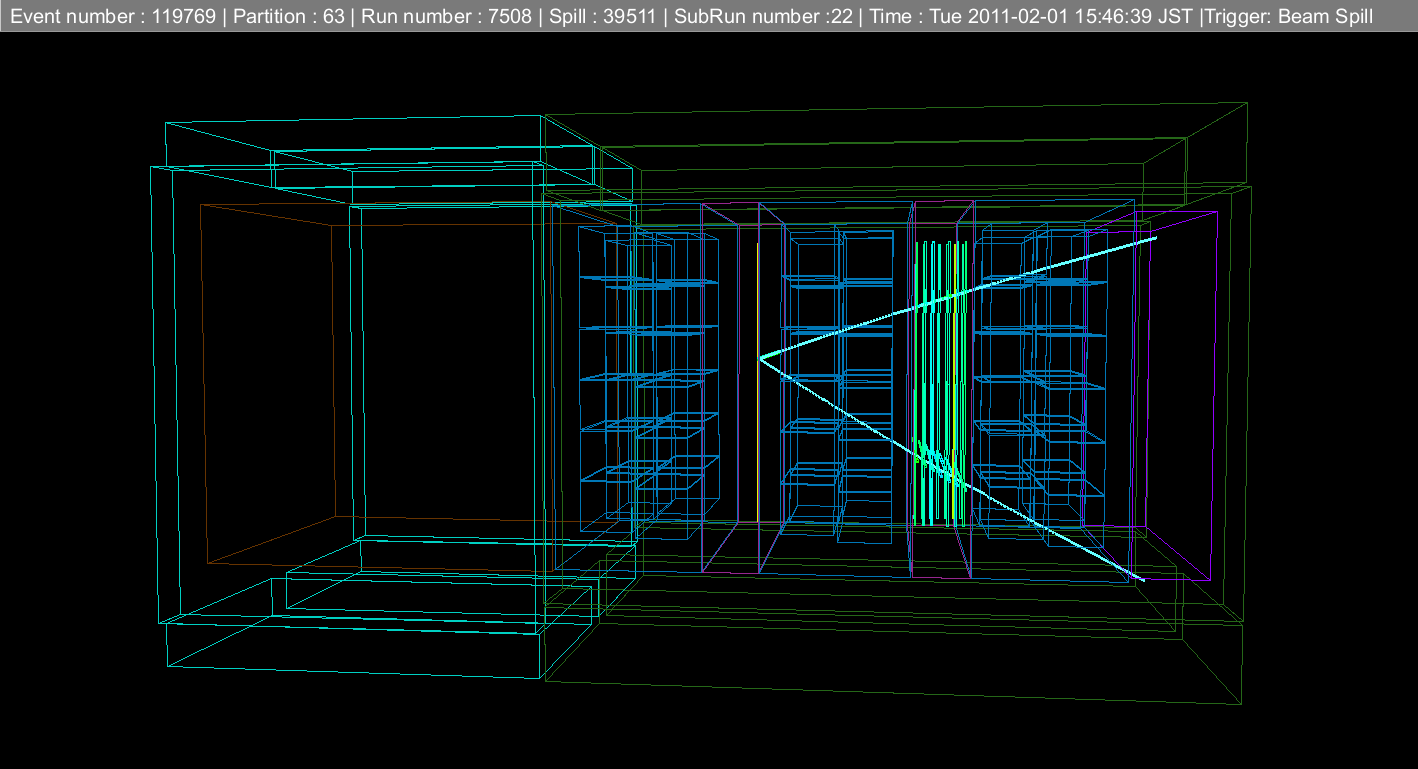
\includegraphics[width=\textwidth, trim={50mm 30mm 50mm 40mm}, clip]{figures/numu/evtdisplay/CC1pi_7508_22_119769_perpX0Z_all}
			\caption{Side-view}
		\end{subfigure}
		\begin{subfigure}[t]{0.49\textwidth}
			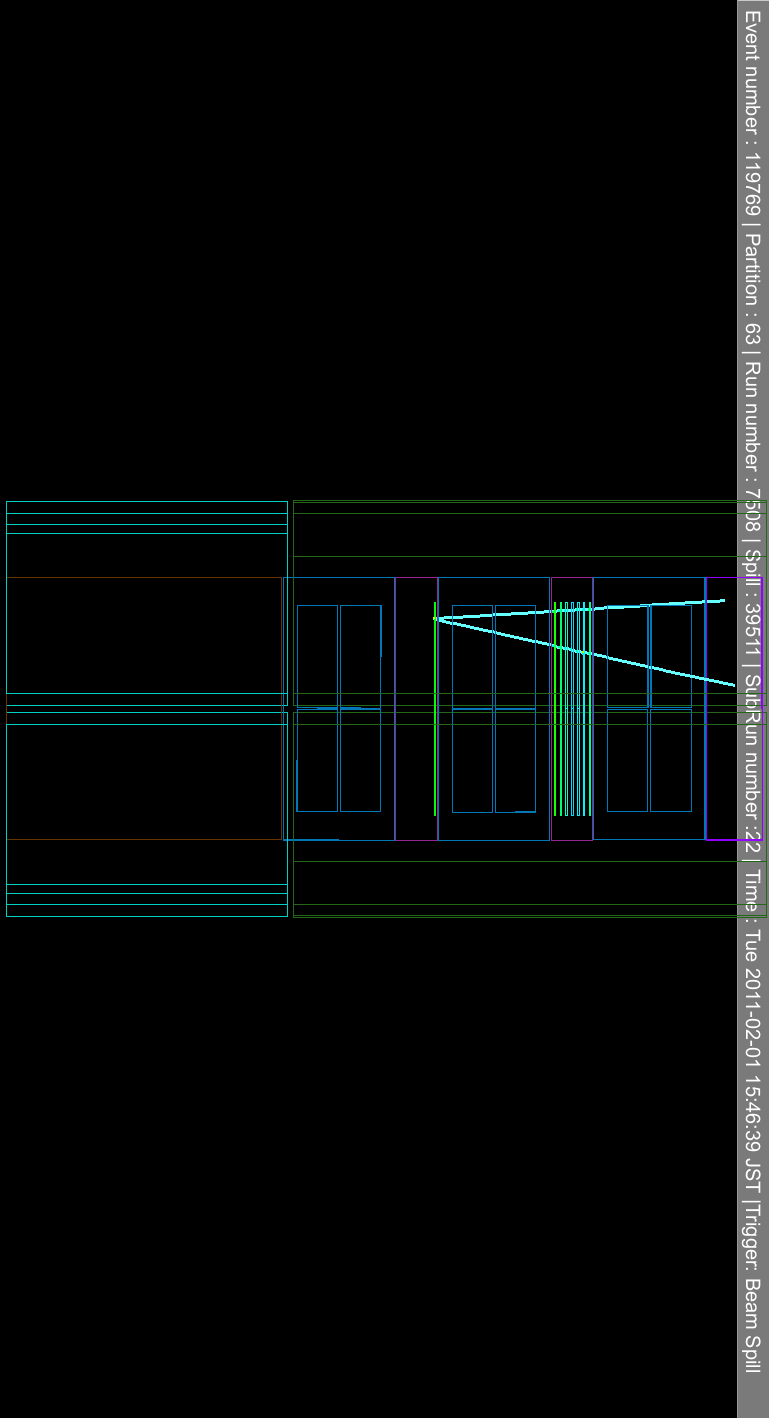
\includegraphics[width=\textwidth, trim={0mm 170mm 10mm 170mm}, clip]{figures/numu/evtdisplay/CC1pi_7508_22_119769_ortX0Z_all}
			\caption{Top-view}
		\end{subfigure}
		\caption{True FGD1 CC1$\pi$ event display in ND280}
		\label{fig:cc1pi_evtdisplay}
	\end{figure}
	
	\item \textbf{CCOther}: All events with one negative muon candidate which are not classified as CC0$\pi$ or CC$1\pi$ fall into this sample. Events with one or more reconstructed negative pion(s), or one or more neutral pion(s) reconstructed as electron or positron candidates in the TPC, are thereby selected. Event with more than one positive pion based on the TPC and FGD pion counting criteria are also accepted. The selection contains mostly multi-$\pi$, DIS and CC$1\pi^0$ interactions. An example event display is shown in \autoref{fig:ccoth_evtdisplay}.
	\begin{figure}[h]
		\begin{subfigure}[t]{0.49\textwidth}
			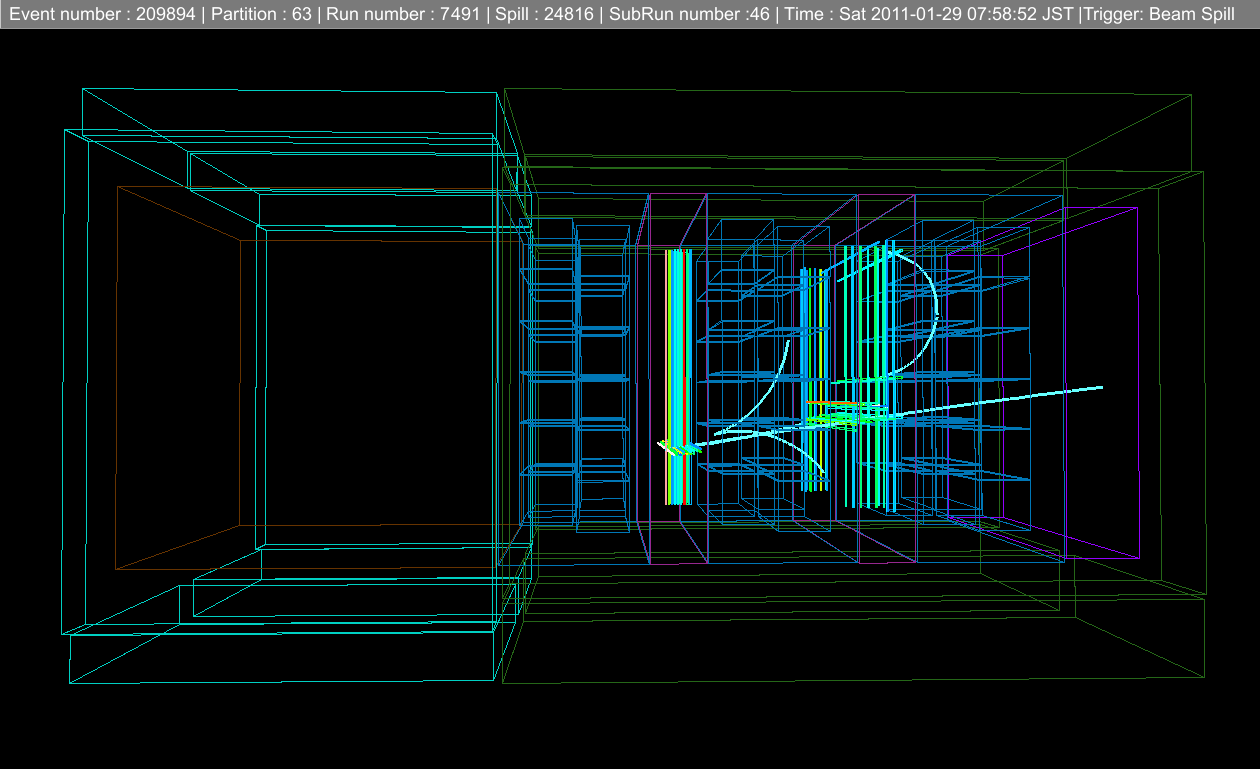
\includegraphics[width=\textwidth, trim={20mm 30mm 20mm 30mm}, clip ]{figures/numu/evtdisplay/CCOthers_7491_46_209894_perX0Z_all}
			\caption{Side-view}
		\end{subfigure}
		\begin{subfigure}[t]{0.49\textwidth}
			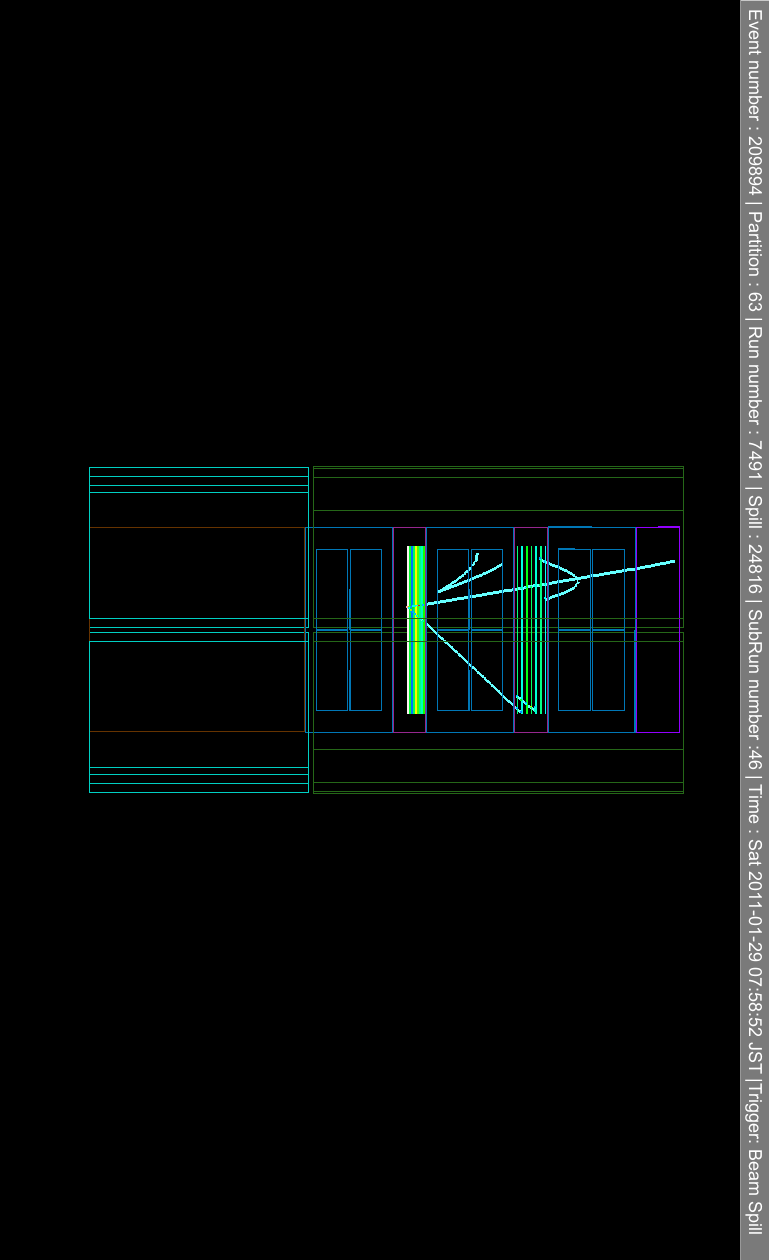
\includegraphics[width=\textwidth, trim={3cm 16cm 3cm 16cm}, clip]{figures/numu/evtdisplay/CCOthers_7491_46_209894_ortX0Z_all}
			\caption{Top-view}
		\end{subfigure}
		\caption{True FGD1 CCOther event display in ND280}
		\label{fig:ccoth_evtdisplay}
	\end{figure}
\end{itemize}

\subsection{\numubar in RHC}
\label{sec:numubar_sel}
The anti-neutrino CC1Track and CCNTrack selections have the same event quality and fiducial volume cut as the neutrino selection, and the muon candidate track is required to pass through the TPC downstream of the struck FGD. The highest momentum track is required to be the highest momentum positive track for its muon PID. The selections generally have a larger background of ``wrong-sign'' events: $\nu_x$ interactions producing $x^-$ which are identified as $\mu^+$, and $\nu_x$ interactions producing a $\pi^+$ which may be identified as the lepton candidate. Hence, the selection cuts proceed differently:
\begin{itemize}
	\item \textbf{Positive multiplicity}: The muon candidate track charge is required to be a highest momentum positive track, which removes a large amount of wrong-sign interactions
	
	\item \textbf{TPC veto}: Veto backwards-going events starting in the FGD and events coming from the P0D and the magnet by utilising the upstream TPCs. If the upstream TPC of an FGD has hits the event is rejected
	
	\item \textbf{Positive muon identification}: The TPC PID outlined for the \numu selections are used to select the positive muon candidate, with the cuts optimised for $\mu^+$. 
	
	$\mathcal{L}_{MIP}$ is defined identically to \autoref{eq:tpc_track_mip} although the cut is now placed at 0.9, and still applies only to particles with $p < 500\text{ MeV}$. The muon likelihood cut is modified to $0.1 < \mathcal{L}_\mu < 0.7$ which removes protons and positive pions from the \numu background. The upper bound at 0.7 is present to reject low energy wrong-sign muons, which may be misidentified as positive tracks. The likelihood distributions and impact of these cuts are shown in \autoref{fig:numubar_likelihood} and \autoref{fig:numubar_likelihood_sel} for the selected lepton candidate. \autoref{fig:numubar_pulls} shows the TPC PID pulls for run5+6.
\end{itemize}

\begin{figure}[h]
	\begin{subfigure}[t]{0.49\textwidth}
		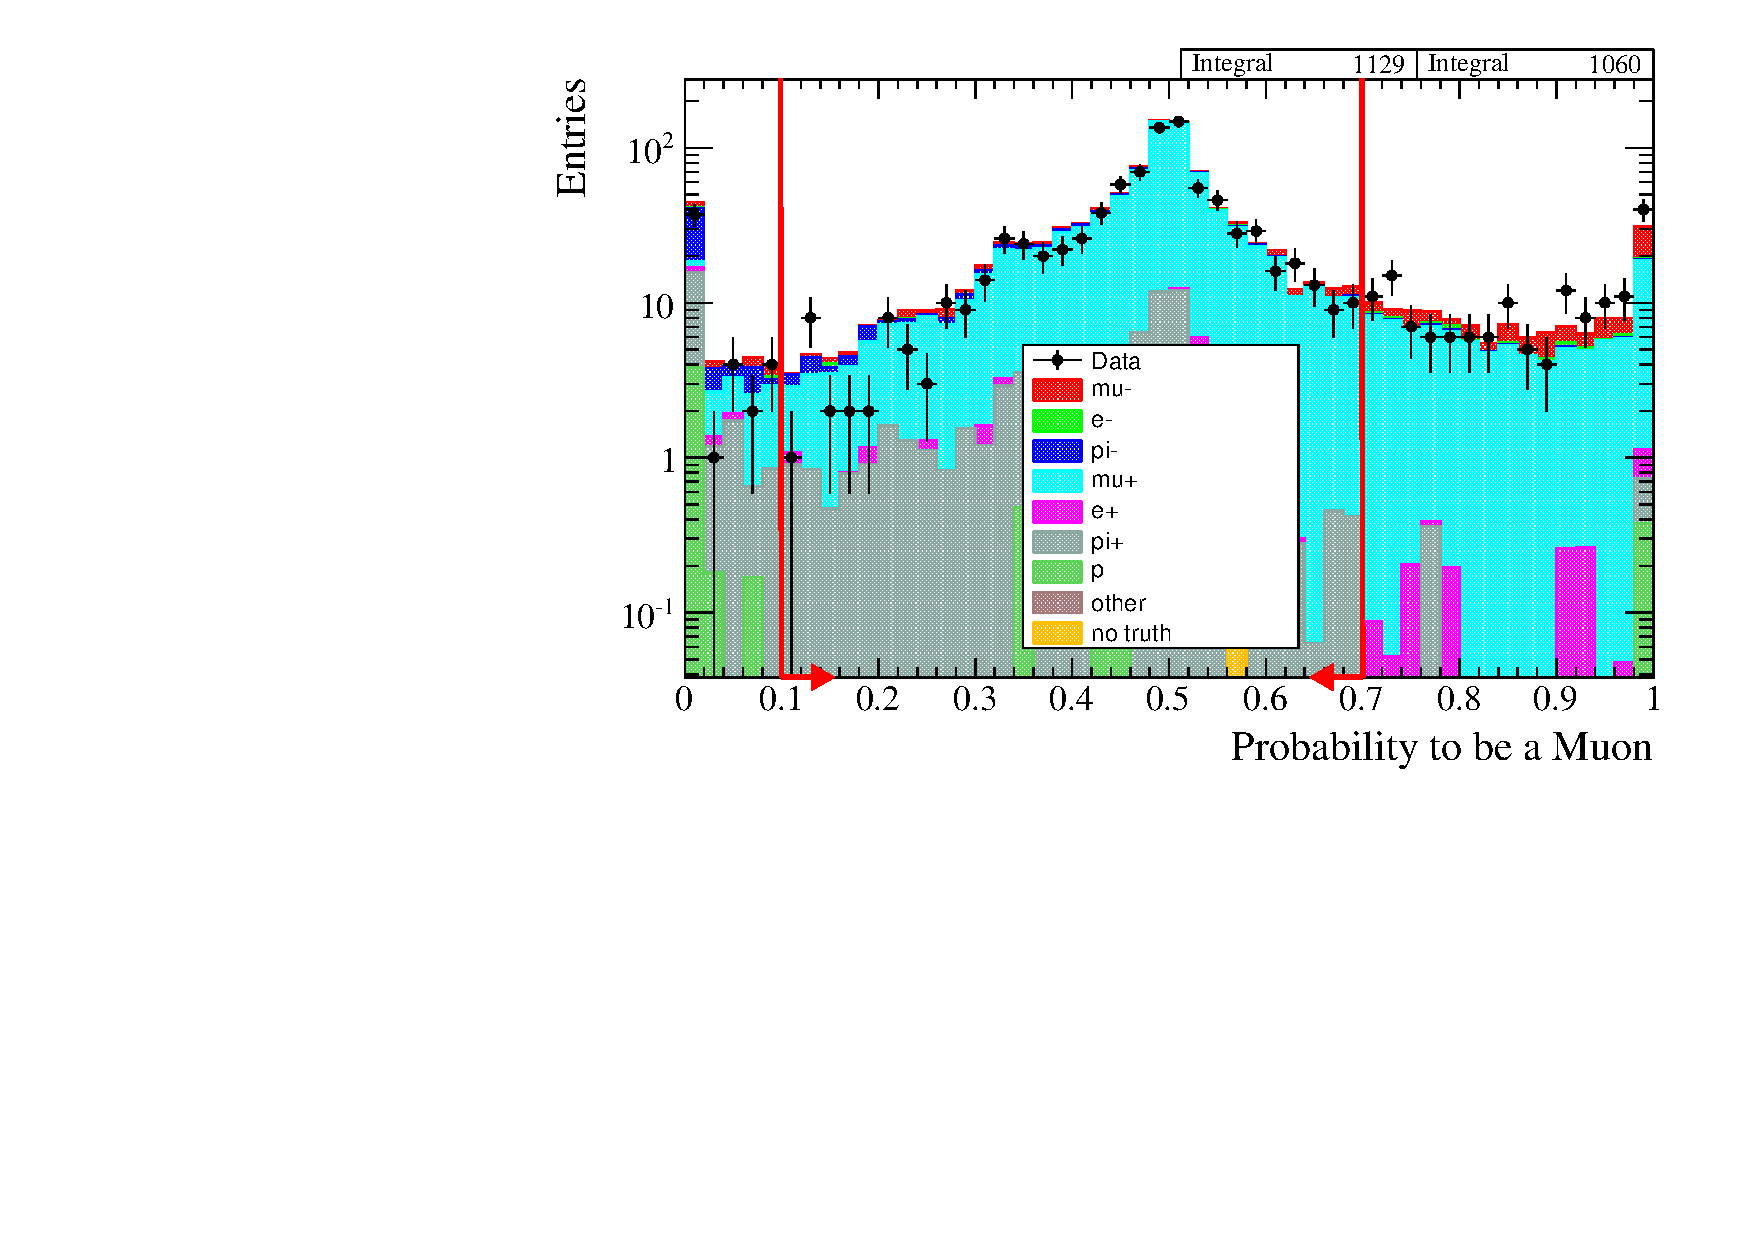
\includegraphics[width=\textwidth]{figures/numu/Cuts/numubar/likemu_numubar}
		\caption{$\mathcal{L}_\mu$}
	\end{subfigure}
	\begin{subfigure}[t]{0.49\textwidth}
		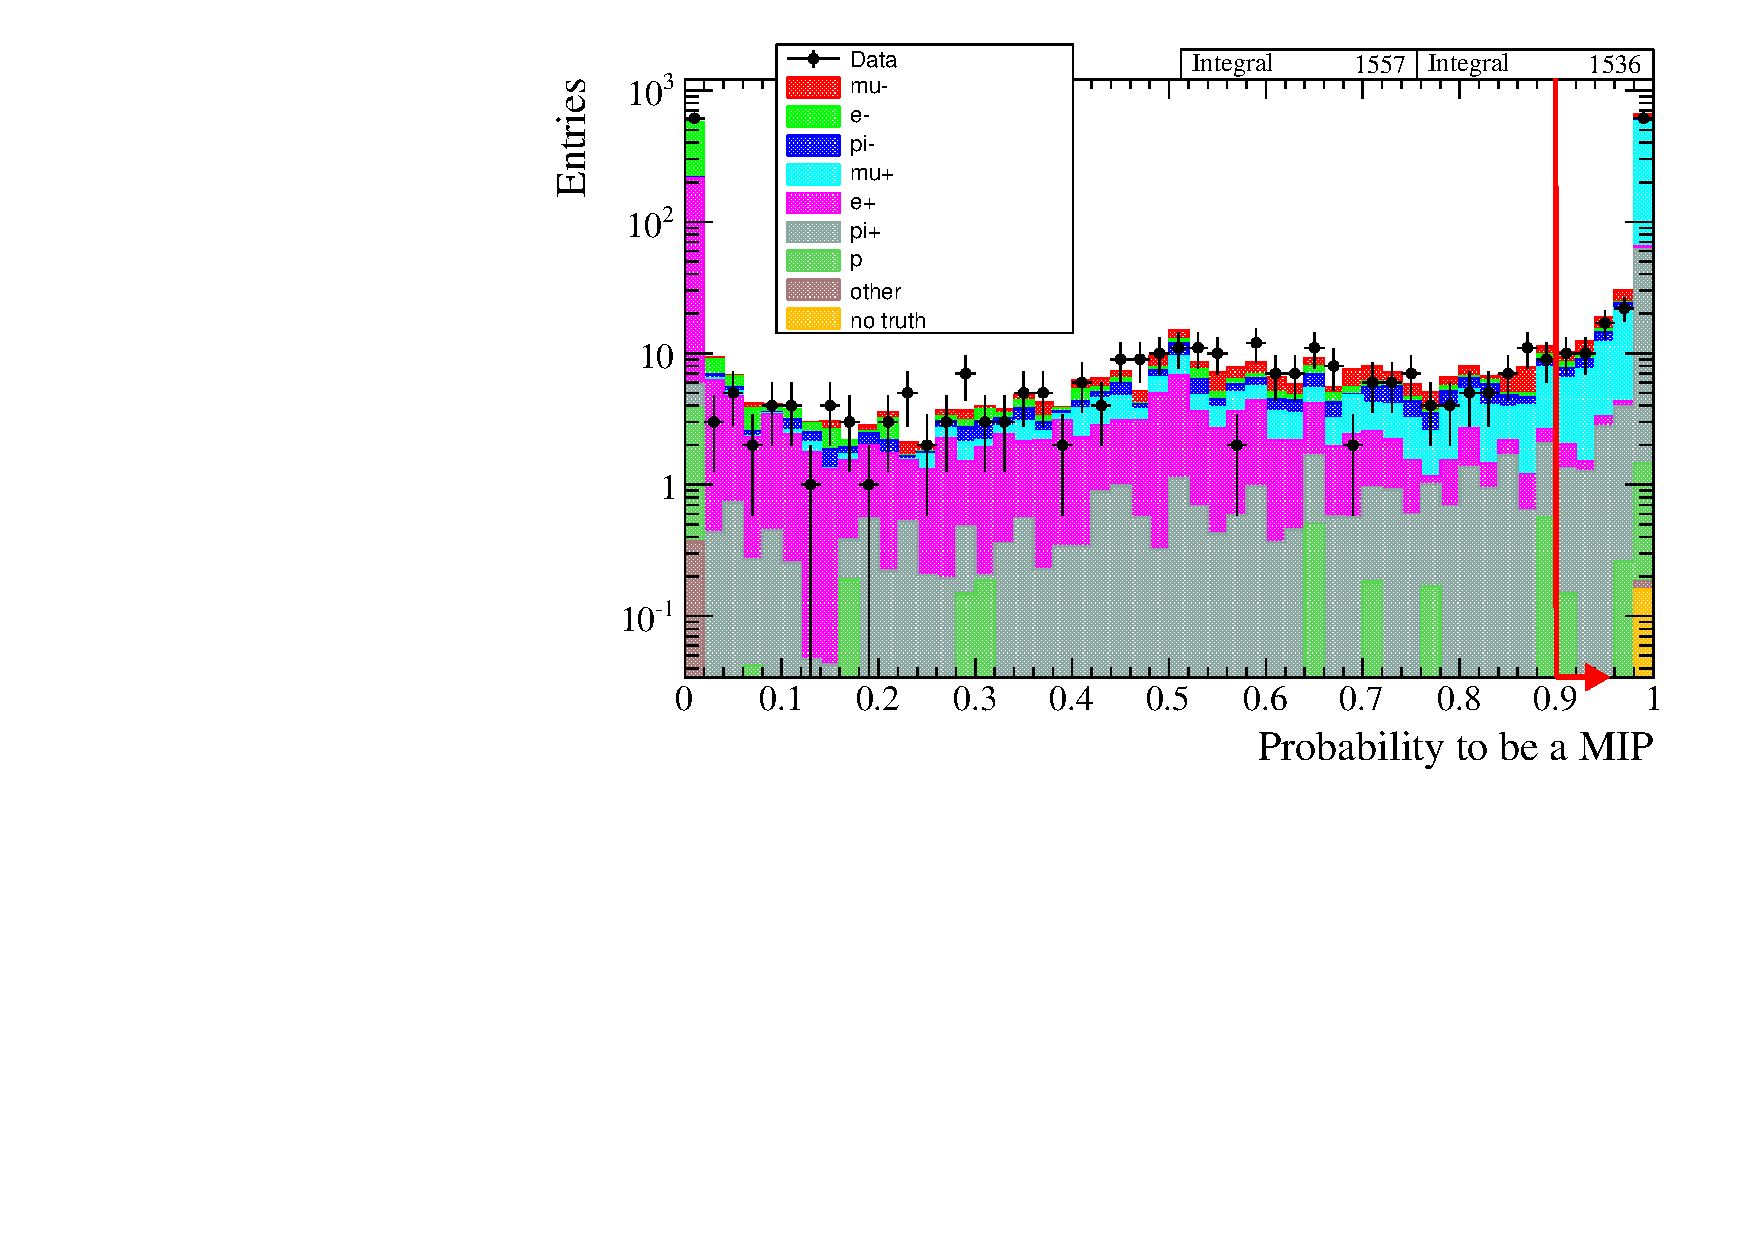
\includegraphics[width=\textwidth]{figures/numu/Cuts/numubar/likemip_numubar}
		\caption{$\mathcal{L}_{MIP}$}
	\end{subfigure}
	\caption{Likelihood distributions for $\mu$ and MIP using run5+6 \numubar data, used in \numubar RHC selections}
	\label{fig:numubar_likelihood}
\end{figure}

\begin{figure}[h]
	\begin{subfigure}[t]{0.49\textwidth}
		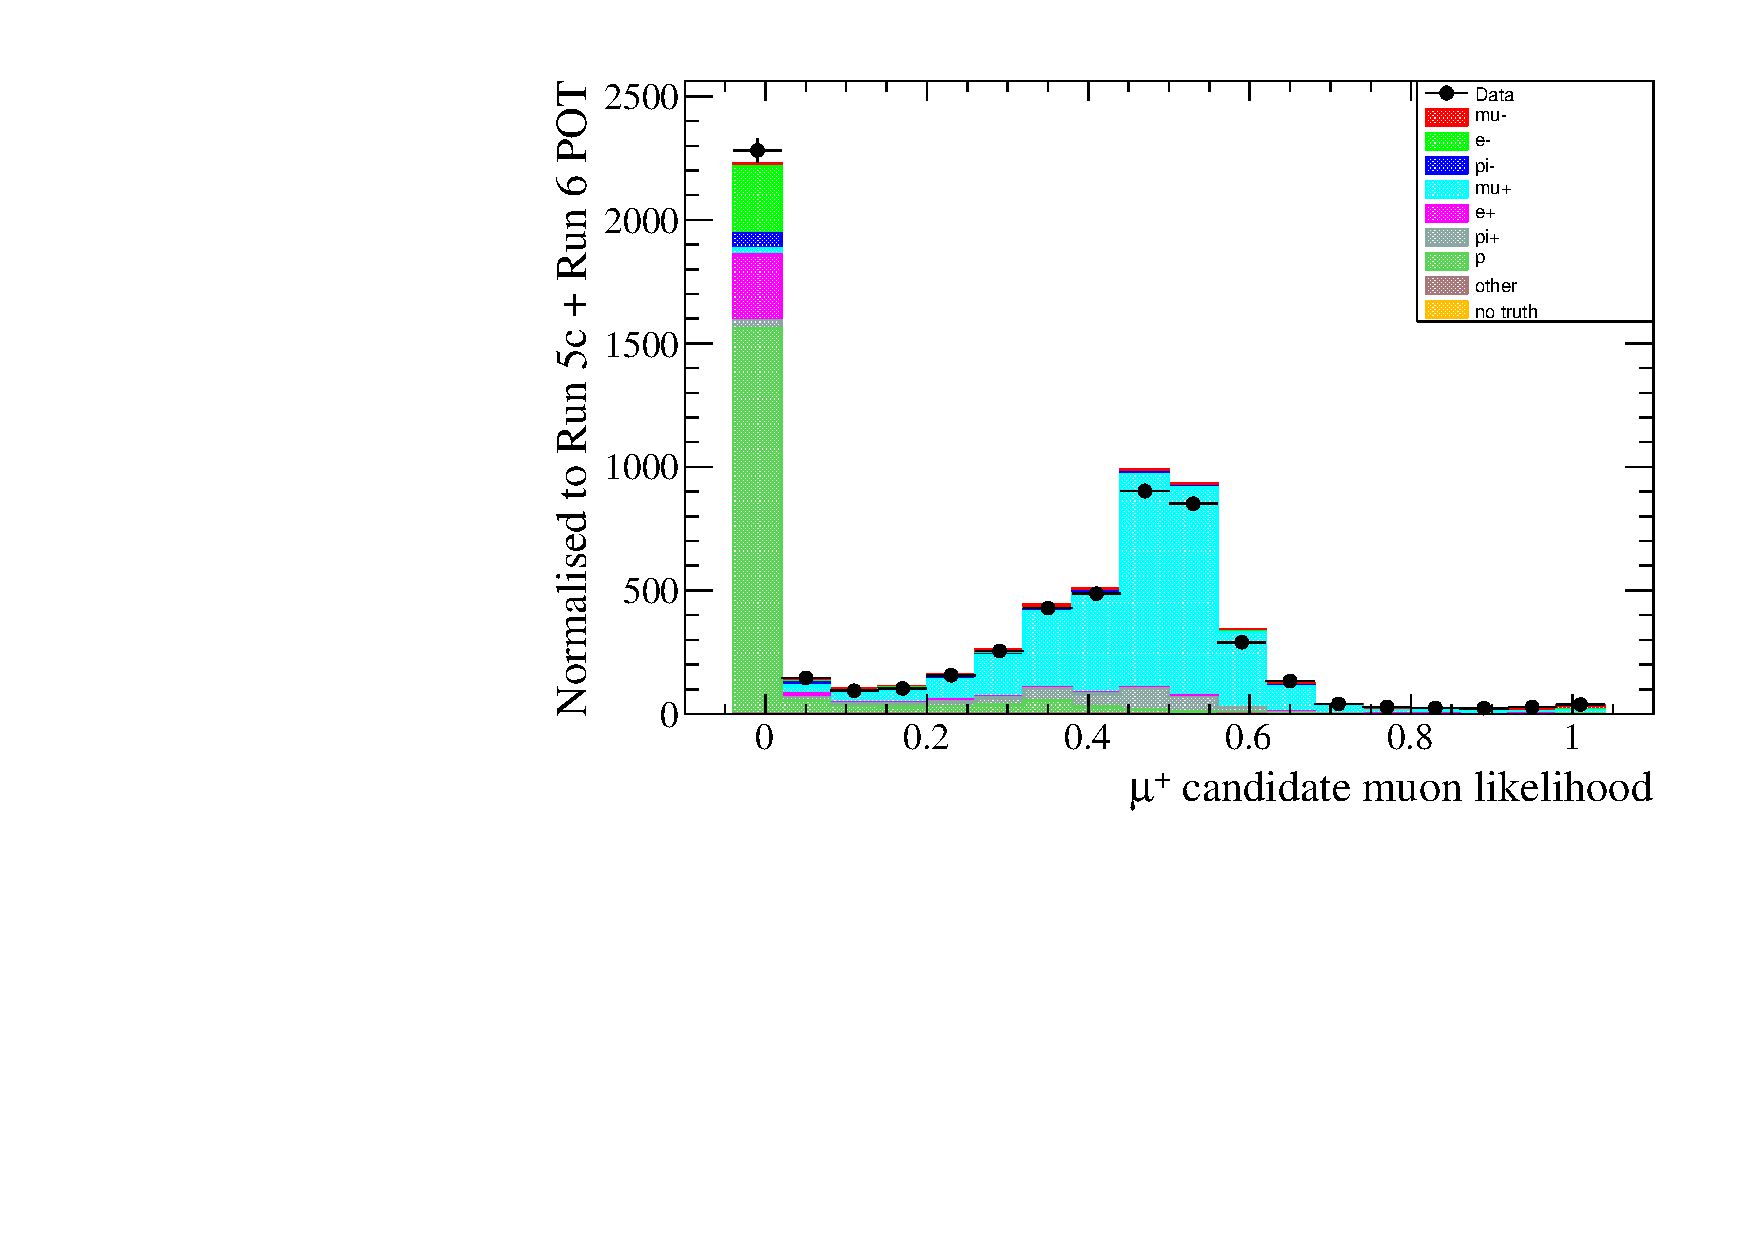
\includegraphics[width=\textwidth]{figures/numu/Cuts/numubar/selmu_likemu_particle}
		\caption{$\mathcal{L}_\mu$}
	\end{subfigure}
	\begin{subfigure}[t]{0.49\textwidth}
		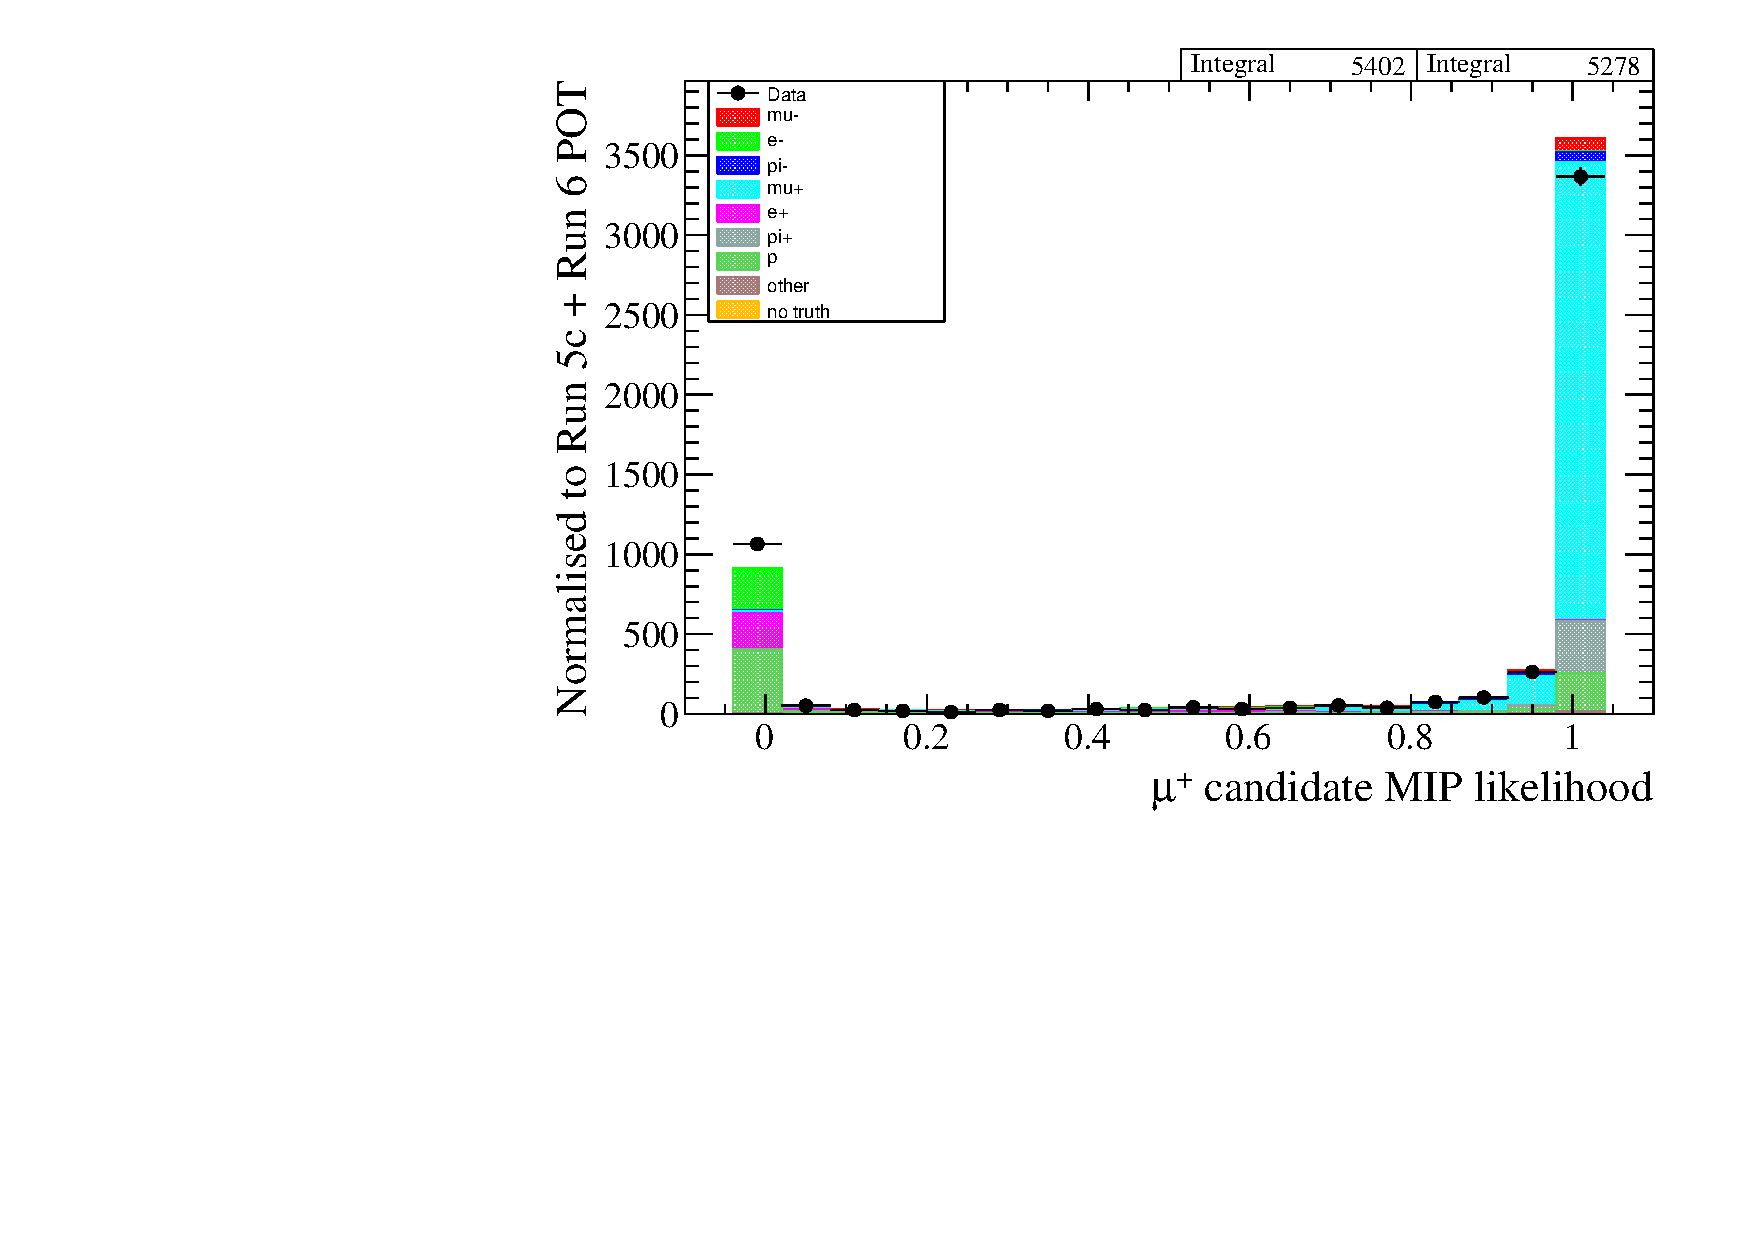
\includegraphics[width=\textwidth]{figures/numu/Cuts/numubar/selmu_likemip_particle}
		\caption{$\mathcal{L}_{MIP}$}
	\end{subfigure}
	\caption{Likelihood distributions for the selected lepton candidate using run5+6 \numubar data, used in \numubar RHC selections}
	\label{fig:numubar_likelihood_sel}
\end{figure}

\begin{figure}[h]
	\begin{subfigure}[t]{0.32\textwidth}
		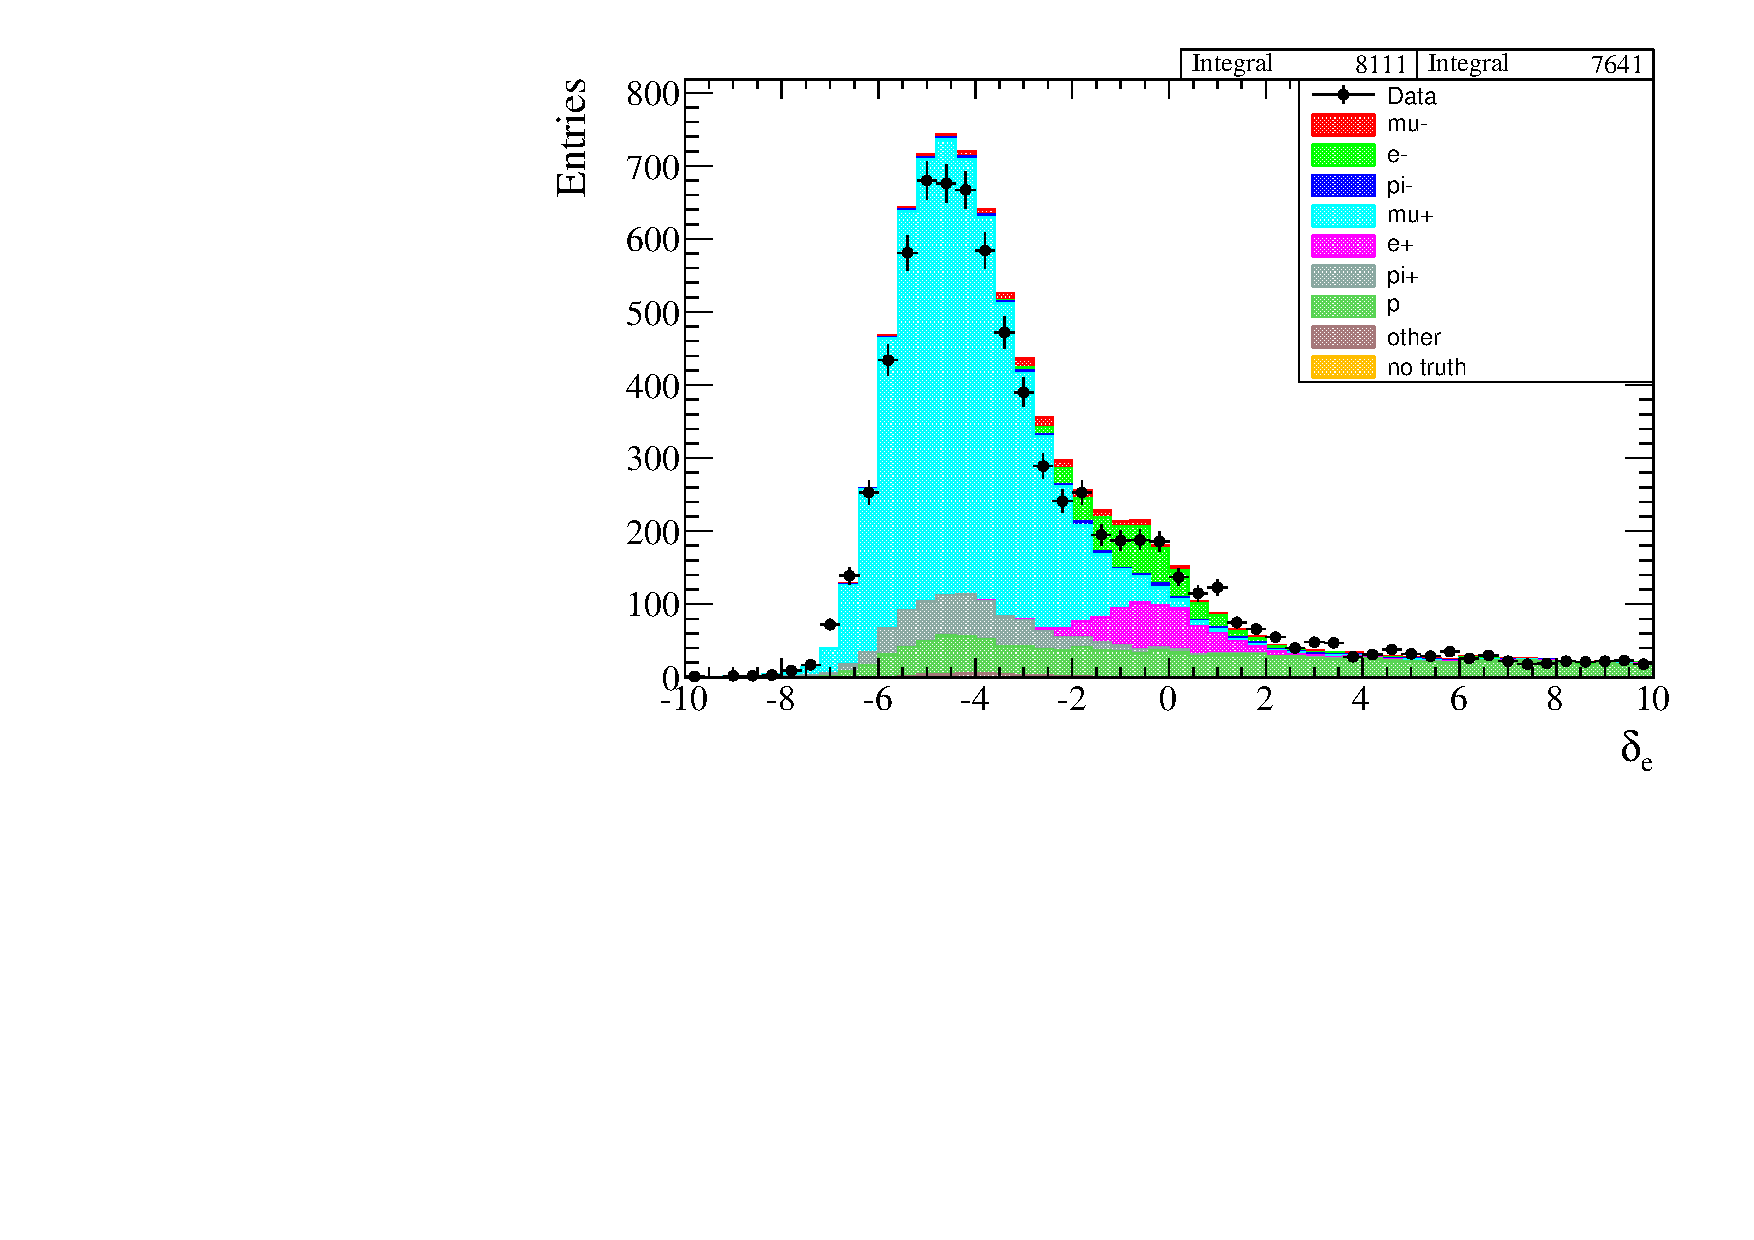
\includegraphics[width=\textwidth]{figures/numu/Cuts/numubar/presel_pullele_part}
		\caption{$\delta_e$}
	\end{subfigure}
	\begin{subfigure}[t]{0.32\textwidth}
		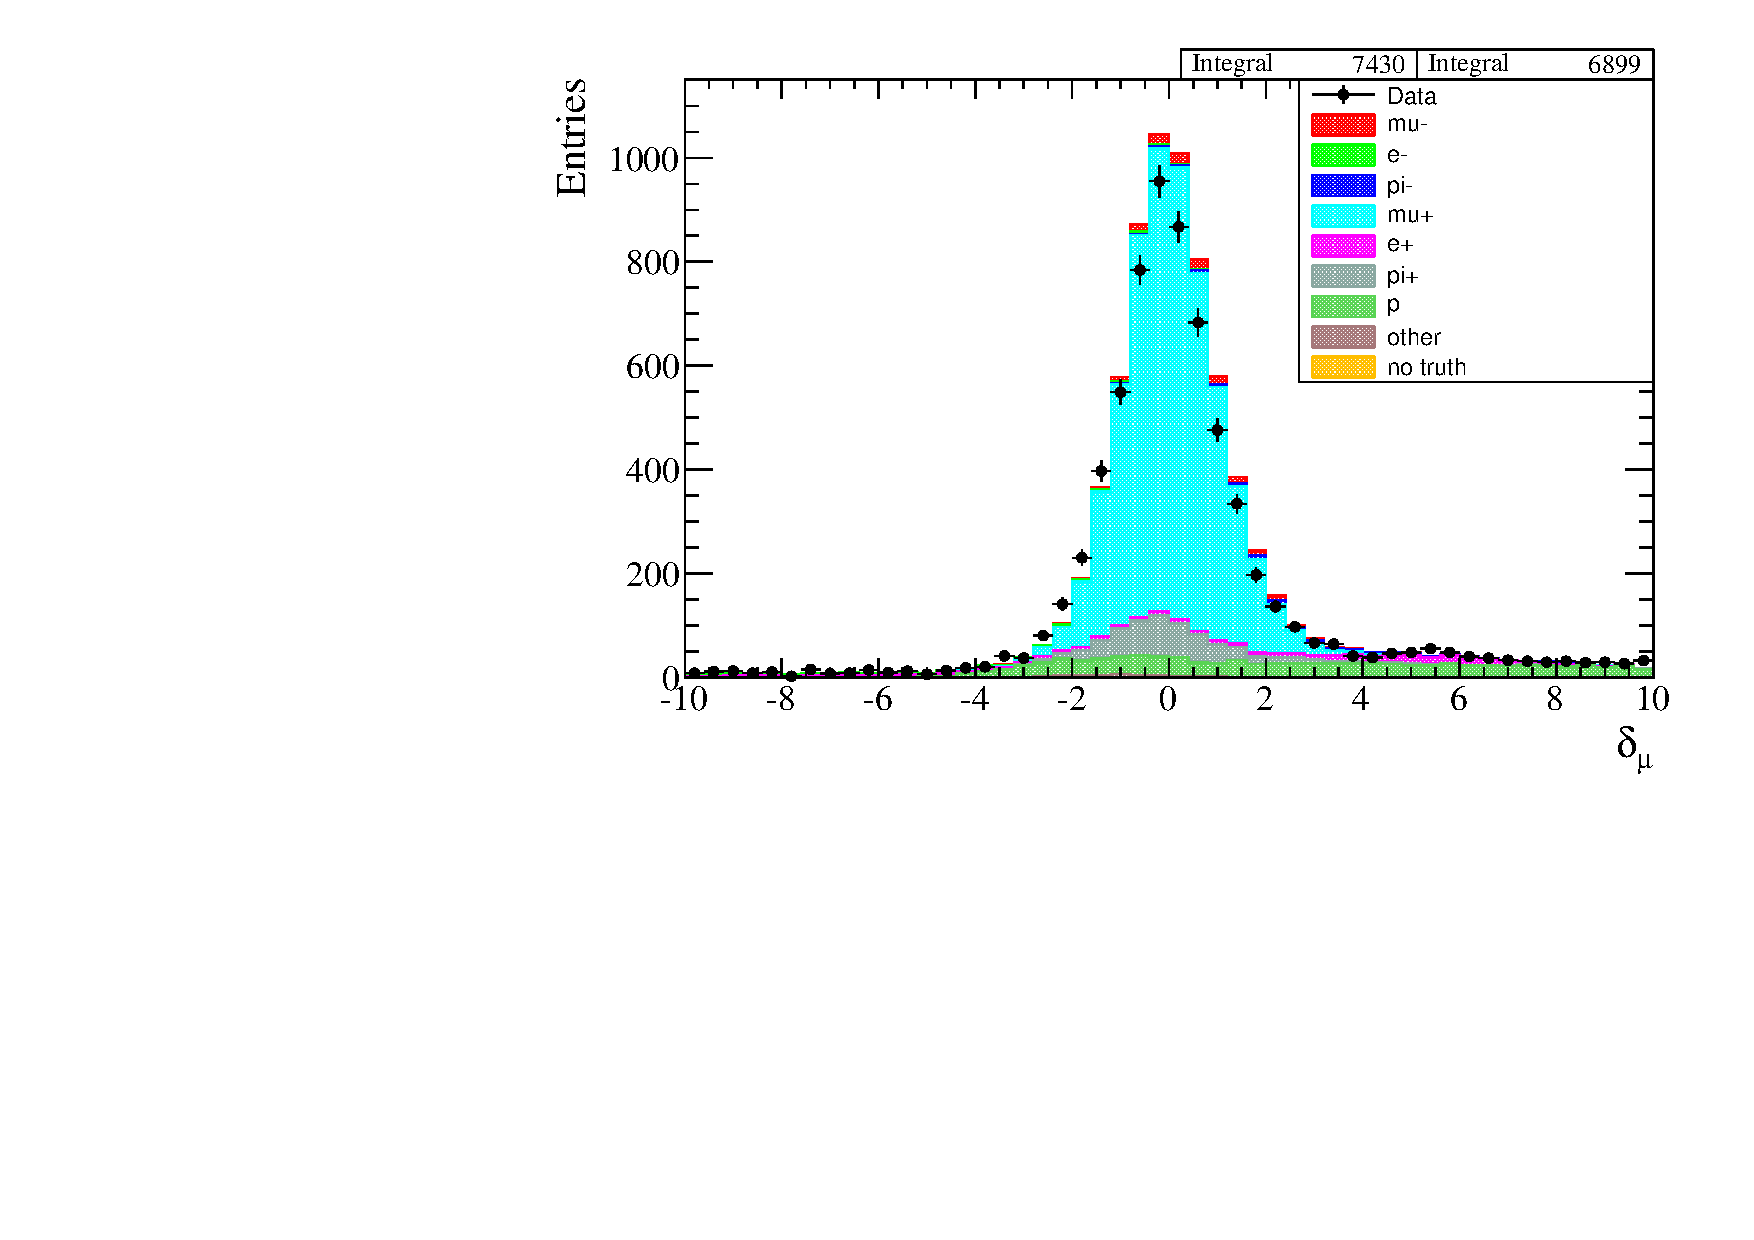
\includegraphics[width=\textwidth]{figures/numu/Cuts/numubar/presel_pullmu_part}
		\caption{$\delta_\mu$}
	\end{subfigure}
	\begin{subfigure}[t]{0.32\textwidth}
		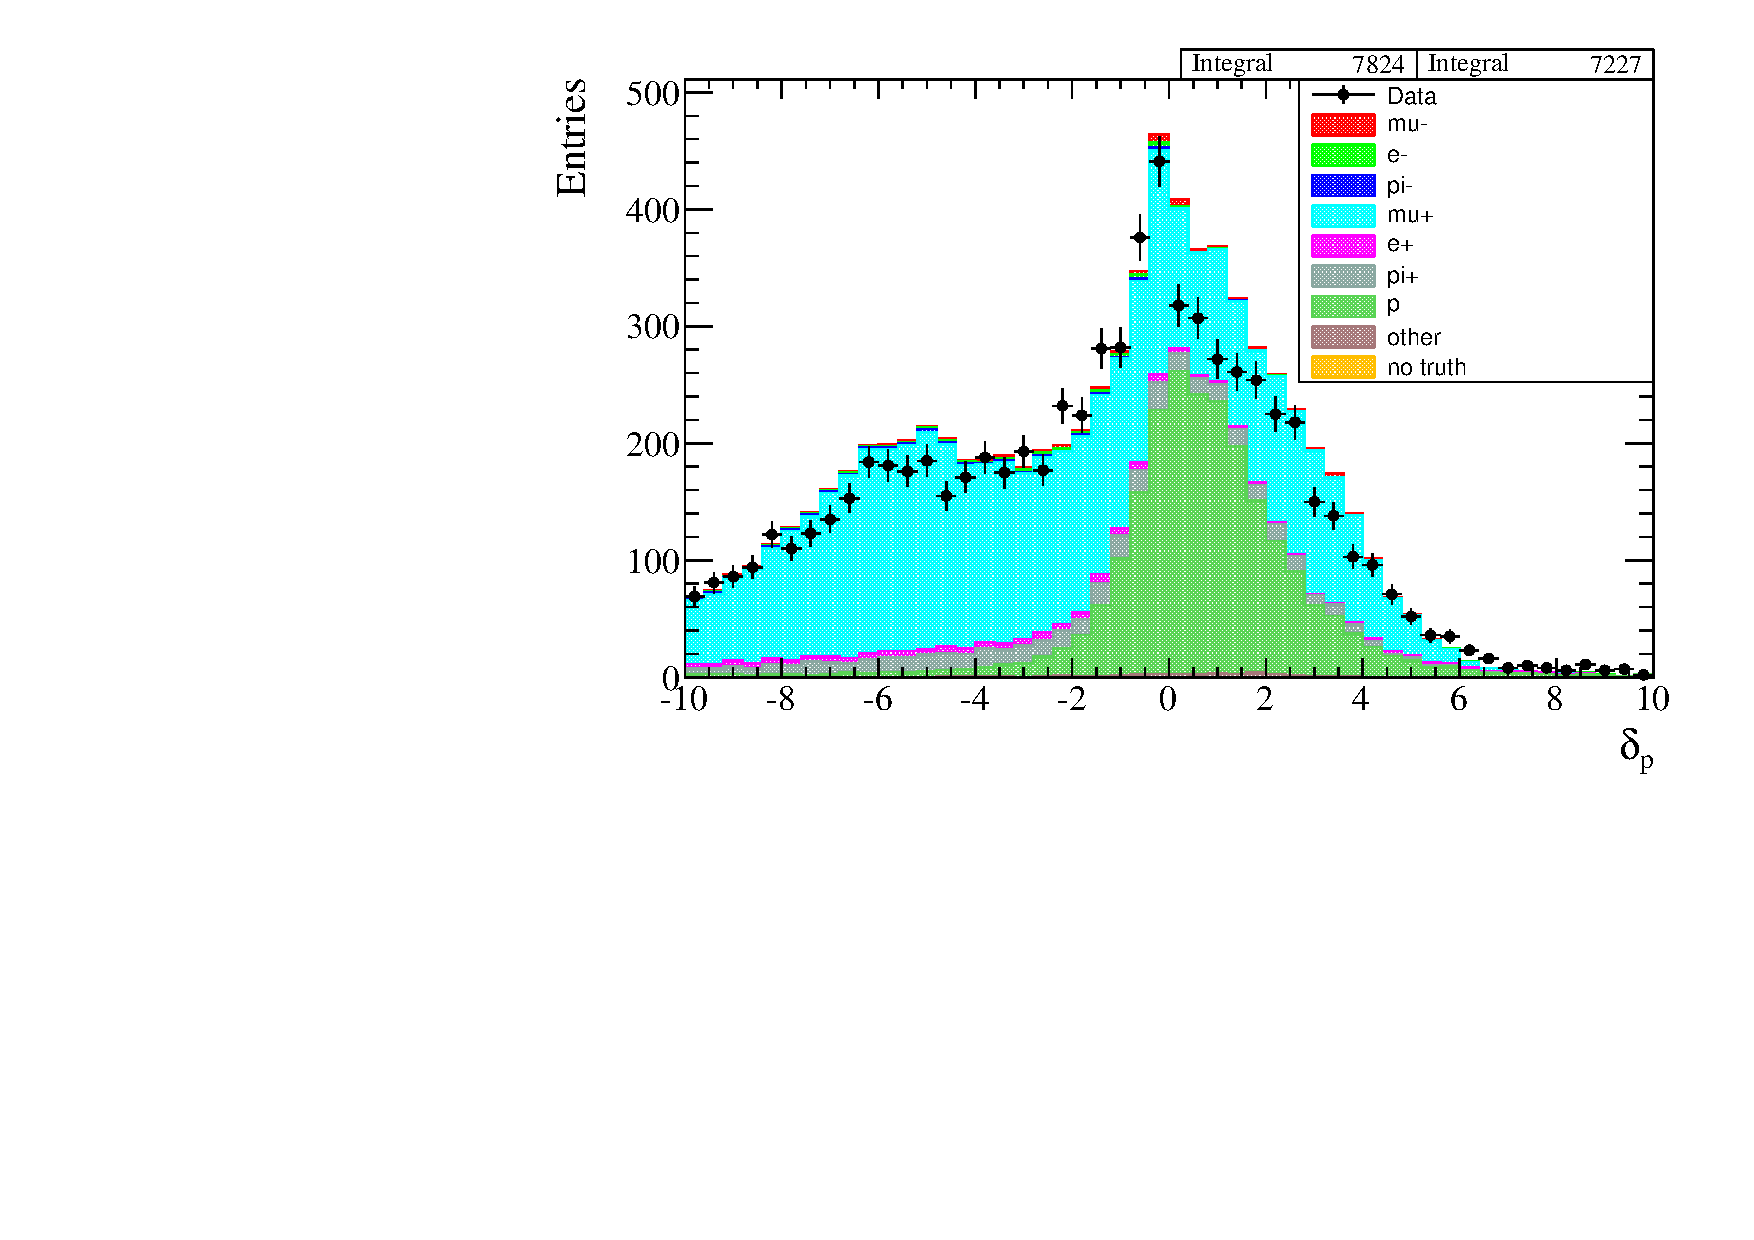
\includegraphics[width=\textwidth]{figures/numu/Cuts/numubar/presel_pullp_part}
		\caption{$\delta_p$}
	\end{subfigure}
	\caption{Pulls ($\delta$) used in the TPC PID used in \numubar RHC selections}
	\label{fig:numubar_pulls}
\end{figure}

Once the \numubar CC-inclusive selection is run the aforementioned pion reconstruction is applied. The \numubar CC1Track selection has one positive muon and does not have any charged or neutral pions in the final state. The \numubar CC1Track selection has a higher efficiency in selecting the muon candidate than the \numu CC0$\pi$ selection from the \numubar resonant interactions producing a $\pi^-$, not a $\pi^+$, which can capture on the nucleus and so do not leave a track to be (falsely) identified as a muon candidate. The \numubar CCNTrack selection contains the remaining particles passing the \numubar CC-inclusive selection, containing at least one neutral or charged pion.

\subsection{\numu in RHC}
\label{sec:numu_in_nubar_sel}
In RHC running there is a large fraction of \numu interactions, owing mostly to the larger \numu cross-section. The same pre-selection cuts are applied for the \numu in RHC selection as for the previous selections.

The CC-inclusive selection proceeds by:
\begin{itemize}
	\item \textbf{Negative multiplicity}: The highest momentum track is required to be the highest momentum negative track, which starts the seeding track. The $\mu^-$ identification uses the TPC PID on the highest momentum negative track. 
	
	\item \textbf{TPC PID}: The PID proceeds by the MIP requirement in \autoref{eq:tpc_track_mip} for particles with $p_\mu < 500 \text{ MeV/c}$, accepting candidate tracks with $\mathcal{L}_{MIP} > 0.7$.
	
	Similar to \autoref{sec:numubar_sel}, a lower and upper bound is set $0.1 < \mathcal{L}_\mu < 0.8$, which rejects protons and low momentum $\mu^+$. The effect of these cuts can be seen in \autoref{fig:nu_numubar_likelihood}.
\end{itemize}

\begin{figure}[h]
	\begin{subfigure}[t]{0.49\textwidth}
		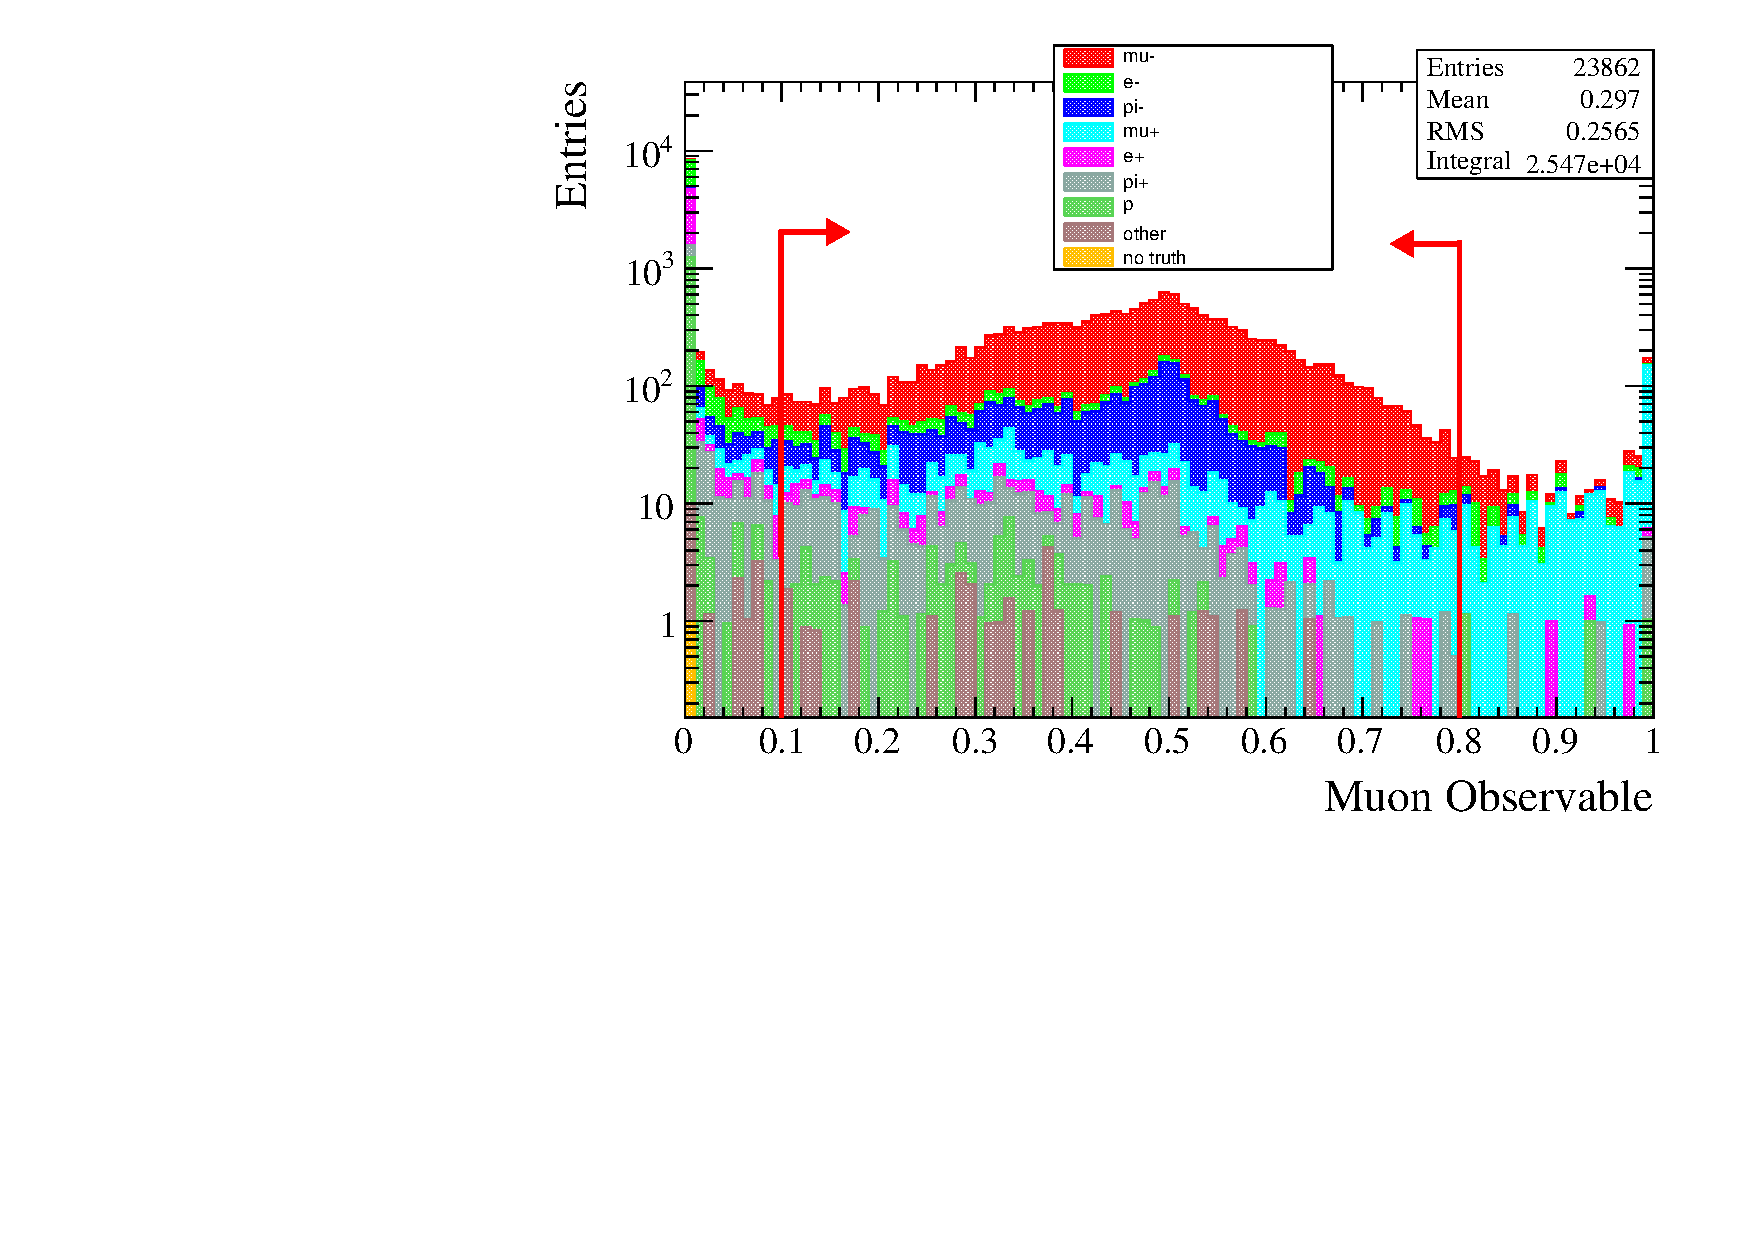
\includegraphics[width=\textwidth]{figures/numu/Cuts/numu_in_numubar/MuonLikelihood_prod6B_NuMuCont_FGD1Only}
		\caption{$\mathcal{L}_\mu$}
	\end{subfigure}
	\begin{subfigure}[t]{0.49\textwidth}
		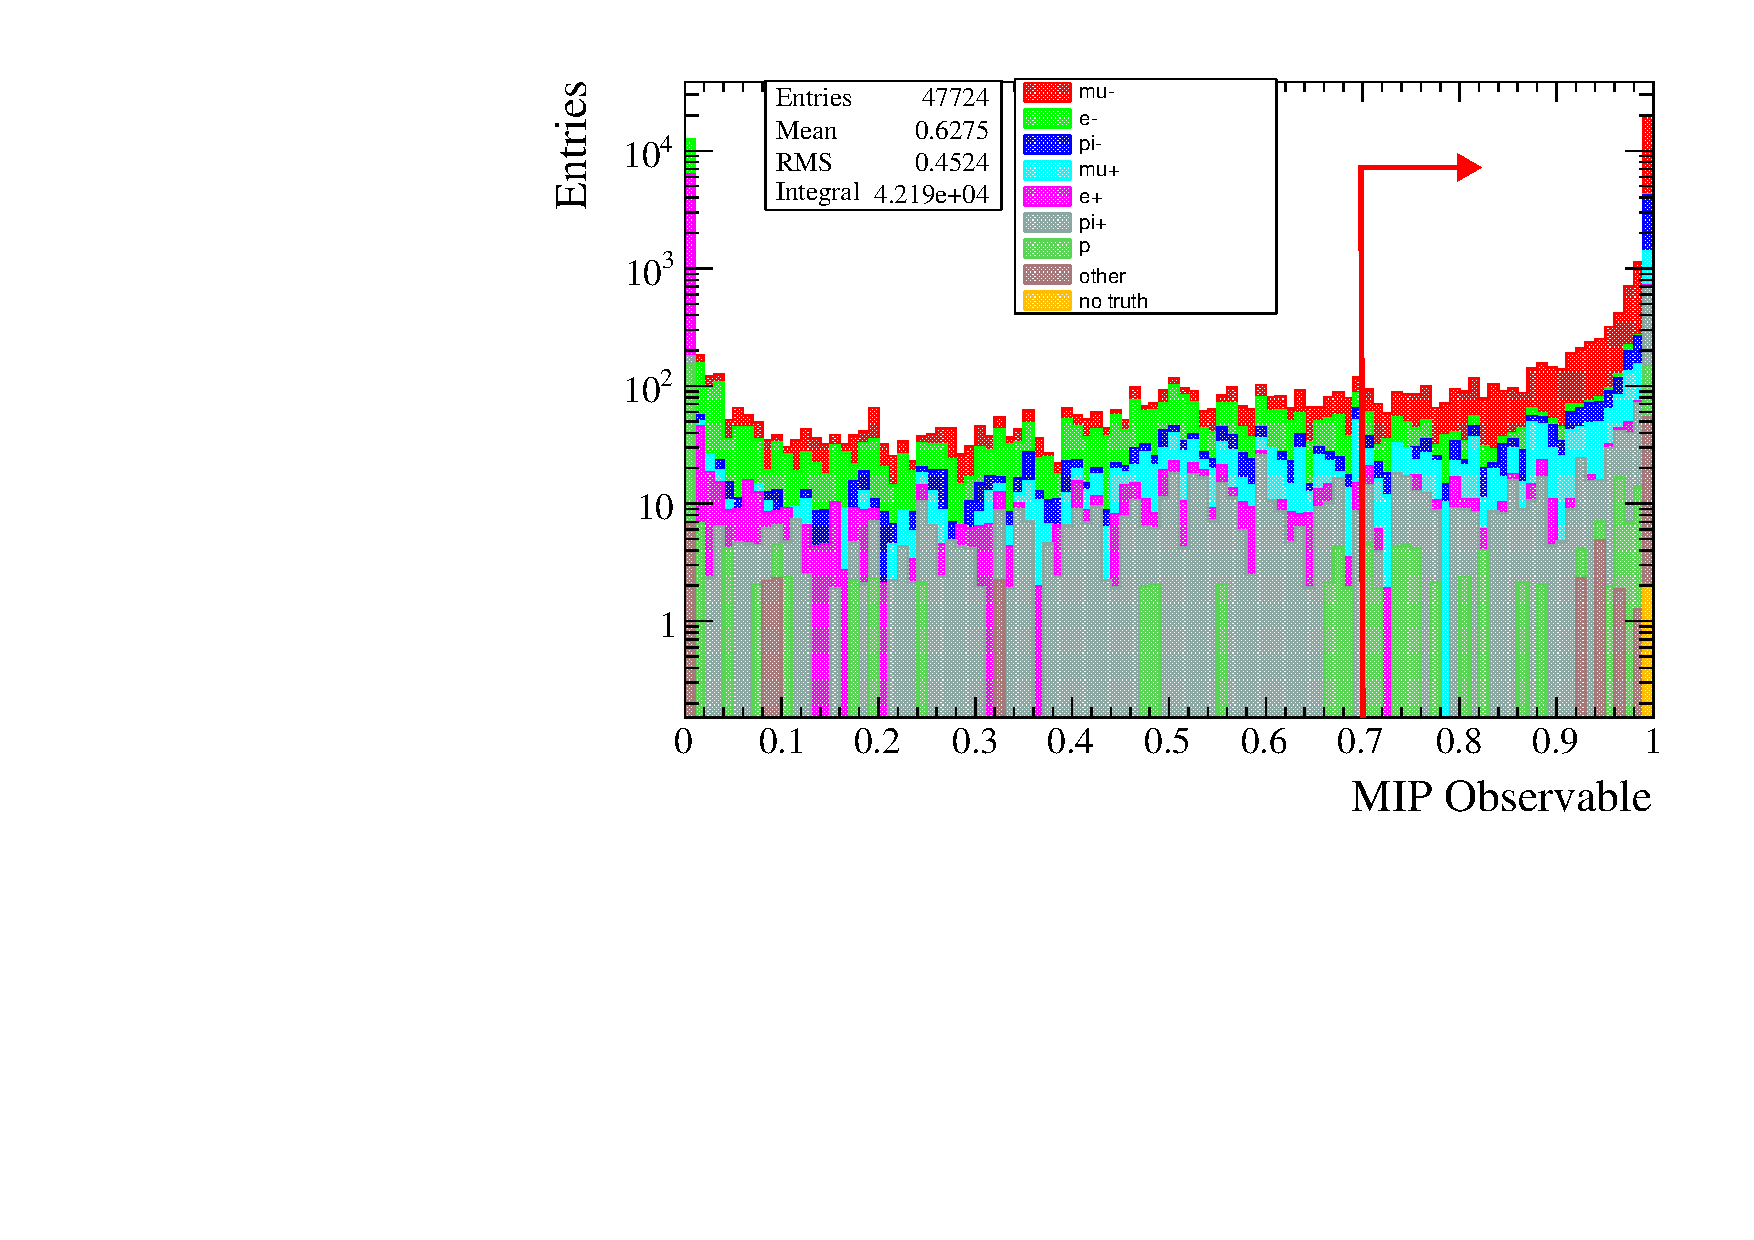
\includegraphics[width=\textwidth]{figures/numu/Cuts/numu_in_numubar/MipLikelihood_LogScale}
		\caption{$\mathcal{L}_{MIP}$}
	\end{subfigure}
	\caption{Likelihood distributions for $\mu$ and MIP using run5+6 \numubar data, used in \numu in RHC selections}
	\label{fig:nu_numubar_likelihood}
\end{figure}

The \numu in RHC selection then breaks down the CC-inclusive selection into CC1Track and CCNTrack, based entirely on the number of TPC-FGD matched tracks. Events with one such reconstructed track enters the CC1Track selection, and events with any other number of tracks regardless of PID, enter the CCNTrack selection. Hence the \numu RHC selection is analogous to the \numubar RHC selection.

A summary of all selections' efficiency and purities is shown in \autoref{tab:eff_pur_summary}. We note $90+\%$ efficiency for CC0$\pi$ and 1 right-sign 1Track efficiencies, with about 75\% purity. As the track multiplicity increases, the efficiencies and purities drop. The NTrack selections in \numubar perform the worst at 55\% efficiency and 45\% purity. For more detail see \autoref{chap:eff_2017}.
\begin{table}[h]
	\centering
	\begin{tabular}{ l | c c }
		\hline
		\hline
		Selection 					   & Efficiency (\%) & Purity (\%) \\ 
		\hline
		\FGDCCNoPi{1}{\numu}           & 93.8  & 75.5  \\% \hline
		\FGDCCNoPi{2}{\numu}           & 93.2  & 73.5  \\% \hline
		\hline
		\FGDCCOnePi{1}{\numu}          & 83.3  & 58.0  \\% \hline
		\FGDCCOnePi{2}{\numu}          & 83.1  & 57.1  \\% \hline
		\hline
		\FGDCCOther{1}{\numu}          & 73.0  & 65.3  \\% \hline
		\FGDCCOther{2}{\numu}          & 73.4  & 64.9  \\% \hline
		\hline
		\FGDCCOneTrk{1}{\numubar}      & 90.0  & 76.7  \\% \hline
		\FGDCCOneTrk{2}{\numubar}      & 89.6  & 76.7  \\% \hline
		\hline
		\FGDCCNTrk{1}{\numubar}   	   & 54.1  & 45.1  \\% \hline
		\FGDCCNTrk{2}{\numubar}        & 53.8  & 43.9  \\% \hline
		\hline
		\FGDCCOneTrk{1}{\numu} in RHC  & 76.5  & 52.2  \\% \hline
		\FGDCCOneTrk{2}{\numu} in RHC  & 74.9  & 51.8  \\% \hline
		\hline
		\FGDCCNTrk{1}{\numu} in RHC    & 73.9  & 60.9  \\% \hline
		\FGDCCNTrk{2}{\numu} in RHC    & 74.2  & 61.4  \\% \hline
		\hline
		\hline
	\end{tabular}
	\caption{Efficiency and purity summary for all selections with the range $0 < p_{reco} < 3\text{ GeV/c}$}
	\label{tab:eff_pur_summary}
\end{table}

\section{Binning the Selections}
\label{sec:binning_2017}
We expect largely similar kinematics across the two FGDs so apply the same binning in reconstructed muon momentum, \pmu, and cosine of the average neutrino-muon angle, \cosmu. The binning for the fit is primarily influenced by MC statistics: we require $\sim 20$ raw MC events per bin (roughly equivalent to 1-2 data events). The momentum resolution is $\sim50\text{ MeV}$ up to 1 GeV and the angular resolution $\sim 2\degree$, seen in \autoref{appendix:detector_resolution}.

The binning in \pmu (MeV/c) \cosmu for each sample is shown below. The FHC selections all have similar binning and has the highest number of bins. The total number of bins is 1624, of which 902 are FHC (six selections) and 722 are RHC (eight selections).
\begin{itemize}
	\item FGD1+2  CC$0\pi$, CC1$\pi$ and CCOther \numu: 154 bins CC0$\pi$, CCOther; 143 bins CC1$\pi$\\
	\pmu: 0, 300, 400, 500, 600, 700, 800, 900, 1000, 1250, 1500, 2000, 3000 (not for CC1$\pi$), 5000, 30000\\
	\cosmu:  -1, 0.6, 0.7, 0.8, 0.85, 0.9, 0.92, 0.94, 0.96, 0.98, 0.99, 1
	
	\item \FGDCCOneTrk{1+2}{\numubar}: 130 bins\\
	\pmu: 0, 400, 500, 600, 700, 800, 900, 1100, 1400, 2000, 10000\\
	\cosmu: -1.0, 0.6, 0.7, 0.8, 0.85, 0.88, 0.91, 0.93, 0.95, 0.96, 0.97, 0.98, 0.99, 1
	
	\item \FGDCCNTrk{1+2}{\numubar}: 77 bins \\
	\pmu: 0, 700, 950, 1200, 1500, 2000, 3000, 10000\\
	\cosmu: -1.0, 0.75, 0.85, 0.88, 0.91, 0.93, 0.95, 0.96, 0.97, 0.98, 0.99, 1
	
	\item \FGDCCnuOneTrk{1+2}{\numu} in RHC: 66 bins\\
	\pmu: 0, 400, 600, 800, 1100, 2000, 10000 \\
	\cosmu: -1.0, 0.7, 0.8, 0.85, 0.9, 0.93, 0.95, 0.96, 0.97, 0.98, 0.99, 1
	
	\item \FGDCCnuNTrk{1+2}{\numu} in RHC: 88 bins\\
	\pmu: 0, 500, 700, 1000, 1250, 1500, 2000, 3000, 10000\\
	\cosmu: -1.0, 0.7, 0.8, 0.85, 0.9, 0.93, 0.95, 0.96, 0.97, 0.98, 0.99, 1
\end{itemize}